\documentclass[a4paper,12pt,svgnames]{report}
\usepackage{preamble}

\chead{}
\rhead{Operációkutatás}
\lhead{Meskó Balázs}
\cfoot{}
\rfoot{\thepage. oldal}
\lfoot{}

\pagestyle{fancy}

\begin{document}

\thispagestyle{empty}
\centerline{\huge \textsc{O}\textsc{perációkutatás}}
\begin{center}

\includegraphics[scale=2]{kepek/me.pdf}\\\medskip
Készítette:\\
{\LARGE Meskó Balázs \\}\medskip
{\large 2011}
\end{center}
\pagebreak

\tableofcontents

%\pagebreak

\chapter{Bevezetés}

Ide majd jön egy kis rizsa arról, hogy mi ez a cucc, meg hogy honnan lett összelopva :-)

A dokumentum \LaTeX-kel készült, az ábrák jelentős része pedig a Ti\textcolor{orange}{\emph{k}}Z csomag segítségével készülhetett el.

\chapter{Lineáris programozás}

\section{A lineáris programozás szimplex módszere}

\subsection{A szimplex módszer}

\subsection{Kiinduló szimplex módszer}

\subsection{Példafeladatok}

\feladatszam Egy üzem kétféle terméket gyárt ($T_1$,$T_2$). A termékek három alkatrész ($A_1$,$A_2$,$A_3$) felhasználásával készülnek. Az első táblázat a termékek szerelési idejét, egységárát és az alkatrészigényüket tartalmazza. Az alkatrészek megmunkálását két gépen végzik ($G_1$,$G_2$). A második táblázat az alkatrészek gépenkénti megmunkálási igényét tartalmazza, és a megmunkálógépek kapacitását. A szerelőüzem kapacitása 220 perc/nap.
\begin{alphanumericlist}
\item Határozza meg a szerelő- és gyártóüzem kapacitását nem meghaladó napi termelést úgy, hogy az árbevétel maximális legyen!
\item Végezzen érzékenységvizsgálatot az 1. termék egységárára illetve a 2. gép kapacitására!
\item Mennyivel kell megváltoztatni a $G_1$ gép kapacitását, hogy az árbevétel 1\%-kal nőjön?
\end{alphanumericlist} 
\begin{align*}
\begin{tabular}{c|ccc|c|c|}
\multicolumn{1}{c}{}&\multicolumn{1}{c}{$A_1$}&\multicolumn{1}{c}{$A_2$}&
\multicolumn{1}{c}{$A_3$}&\multicolumn{1}{c}{Szerelés}&
\multicolumn{1}{c}{Egységár}\\\cline{2-6}
$G_1$&$1$&$0$&$2$&$2$&$27$\\
$G_2$&$0$&$1$&$1$&$1$&$8$\\\cline{2-6}
\end{tabular}&&
\begin{tabular}{c|ccc|c|}
\multicolumn{1}{c}{}&\multicolumn{1}{c}{$A_1$}&\multicolumn{1}{c}{$A_2$}&
\multicolumn{1}{c}{$A_3$}&\multicolumn{1}{c}{Kapacitás}\\\cline{2-5}
$G_1$&$1$&$0$&$1$&$240$\\
$G_2$&$7$&$1$&$1$&$630$\\\cline{2-5}
\end{tabular}
\end{align*}

\begin{megoldas}
Először is a megoldáshoz fel kell írnunk a matematikai modellt, amelyhez ki kell hámoznunk az adatokat a táblázatokból:
\begin{alignat*}{6}
1\cdot 1x_1&+&0\cdot0x_2&+&1\cdot2x_3&+&1\cdot0x_1&+&0\cdot1x_2&+&1\cdot1x_3&\leq240\\
7\cdot1x_1&+&1\cdot0x_2&+&1\cdot2x_3&+&7\cdot0x_1&+&1\cdot1x_2&+&1\cdot1x_3&\leq630\\
&&&&&&&&2x_1&+&1x_2&\leq220\\
&&&\mathrlap{27x_1+8x_2\longrightarrow\max!}
\end{alignat*}

azaz
\begin{alignat*}{3}
3x_1&+&x_2&\leq240\\
9x_1&+&2x_2&\leq630\\
2x_1&+&1x_2&\leq220\\
27x_1&+&8x_2&\longrightarrow\max!\\
x_1&,&x_2&\geq0
\end{alignat*}

A következő lépés az LP feladat sztenderdizálása:
\begin{alignat*}{5}
3x_1&+&x_2&+&u_1&=240\\
9x_1&+&2x_2&+&u_2&=630\\
2x_1&+&1x_2&+&u_3&=220\\
&&\mathclap{-27x_1-8x_2\longrightarrow\min!}\\
&&&&&&\mathllap{x_1,x_2,u_1,u_2,u_3\geq0}
\end{alignat*}

\begin{multicols}{2}
\begin{tabular}{c|cc|c|}
\multicolumn{1}{c}{}&\multicolumn{1}{c}{$x_1$}&
\multicolumn{1}{c}{$x_2$}&\multicolumn{1}{c}{}\\\cline{2-4}
$u_1$&  $2$& \circled{$1$}& $220$\\
$u_2$&  $3$& $1$& $240$\\
$u_3$&  $9$& $2$& $630$\\\cline{2-4}
     & $27$& $8$&   $0$\\\cline{2-4}
\end{tabular}

\begin{tabular}{c|cc|c|}
\multicolumn{1}{c}{}&\multicolumn{1}{c}{$x_1$}&
\multicolumn{1}{c}{$u_1$}&\multicolumn{1}{c}{}\\\cline{2-4}
$x_2$&  $2$&  $1$&   $220$\\
$u_2$&  \circled{$1$}& $-1$&    $20$\\
$u_3$&  $5$& $-2$&   $190$\\\cline{2-4}
     & $11$& $-8$& $-1760$\\\cline{2-4}
\end{tabular}
\end{multicols}\begin{multicols}{2}
\begin{tabular}{c|cc|c|}
\multicolumn{1}{c}{}&\multicolumn{1}{c}{$u_2$}&
\multicolumn{1}{c}{$u_1$}&\multicolumn{1}{c}{}\\\cline{2-4}
$x_2$& $-2$&  $3$&   $180$\\
$x_1$&  $1$& $-1$&    $20$\\
$u_3$& $-5$&  \circled{$3$}&    $90$\\\cline{2-4}
     &$-11$&  $3$& $-1980$\\\cline{2-4}
\end{tabular}

\begin{tabular}{c|cc|c|}
\multicolumn{1}{c}{}&\multicolumn{1}{c}{$u_2$}&
\multicolumn{1}{c}{$u_3$}&\multicolumn{1}{c}{}\\\cline{2-4}
$x_2$&              $3$&           $-1$&    $90$\\
$x_1$&  $-\nicefrac{2}{3}$& $\nicefrac{1}{3}$&    $50$\\
$u_1$&  $-\nicefrac{5}{3}$& $\nicefrac{1}{3}$&    $30$\\\cline{2-4}
     &             $-6$&           $-1$& $-2070$\\\cline{2-4}
\end{tabular}
\end{multicols}

Mivel a $\mathbf{z}-\mathbf{c}$ vektor $\leq0$, ezért megvan az optimális megoldás, amely az $\mathbf{x}=(50,90)$ vektor. A célfüggvény értéke ekkor $-2070$, azonban ez a segédfeladaté! Az eredeti feladatot maximumot keres, így az eredeti célfüggvény értéke $2070$.
\end{megoldas}

\begin{megoldas}
\medskip\hrule\medskip

Az első termék ára $27 \longrightarrow 27+\lambda$. A célfüggvény az alábbi módon változik:
\begin{align*}
(-27-\lambda)x_1-8x_2\longrightarrow\min!&&
(27+\lambda)x_1+8x_2\longrightarrow\max!
\end{align*}

Mivel az $x_1$-hez tartozó paraméter változik, a táblázatban az $x_1$ sorát kell figyelni:
\begin{alignat*}{4}
-6&+&\tfrac{2}{3}\lambda&\leq&0&\qquad\longrightarrow\qquad&\lambda\leq9\\
-1&-&\tfrac{1}{3}\lambda&\leq&0&\qquad\longrightarrow\qquad&\lambda\geq-3\\
\mathclap{z_{\min}=-2070-50\lambda}&&&&&&
\mathclap{z_{\max}=2070+50\lambda}
\end{alignat*}

A második gép kapacitása $630 \longrightarrow 630+\lambda$. Az eredményoszlop eképpen változik:
\begin{alignat*}{5}
90&-&1\lambda&\geq&0&\qquad\longrightarrow\qquad&\lambda&\leq90\\
50&+&\tfrac{1}{3}\lambda&\geq&0&\qquad\longrightarrow\qquad&\lambda&\geq-150\\
30&+&\tfrac{1}{3}\lambda&\geq&0&\qquad\longrightarrow\qquad&\lambda&\geq-90\\
\mathclap{\hskip 0.1cm z_{\min}=-2070-\lambda}&&&&&&&&
\mathclap{\hskip -0.9cm z_{\max}=2070+\lambda}
\end{alignat*}\hrule\medskip

A feladatrész megoldásához először érzékenységvizsgálatot kell végezni. Az első gép kapacitása $240 \longrightarrow 240+\lambda$. Az eredményoszlop az alábbiak szerint alakul:
\begin{alignat*}{5}
90&+&3\lambda&\geq&0&\qquad\longrightarrow\qquad&\lambda&\geq-30\\
50&-&\tfrac{2}{3}\lambda&\geq&0&\qquad\longrightarrow\qquad&\lambda&\leq75\\
30&-&\tfrac{5}{3}\lambda&\geq&0&\qquad\longrightarrow\qquad&\lambda&\leq18\\
\mathclap{\hskip 0.1cm z_{\min}=-2070-6\lambda}&&&&&&&&
\mathclap{\hskip -0.7cm z_{\max}=2070+6\lambda}
\end{alignat*}

Az árbevétel növeléséhez a célfüggvényt értéket kell növelni, tehát:
\begin{align*}
2070+6\lambda&= 2070\cdot1,01\\
\lambda&=3,45
\end{align*}

Ez belefér az érzékenységi intervallumba, a megoldás ekkor $\mathbf{x}=(47,7;100,35)^T$
\end{megoldas}


\feladatszam Egy üzemben három terméket gyártanak, melyek megmunkálása két fázisban -- egy esztergán és egy marógépen -- történik. Az első termék esztergagépen történő megmunkálása 1 perc/db, a marógépen pedig 1 perc/db. A második terméké rendre 3 és 2 perc/db, a harmadiké pedig rendre 1 és 2 perc/db. Az esztergagép kapacitása 90 perc, a marógépé pedig 120 perc. A termékek várható eladási egységára rendre 1, 2 és 3 pénzegység, a tervezett árbevétel pedig 110 pénzegység. A gépek állásidejének költsége rendre 2 és 1 pénzegység/perc.

\begin{alphanumericlist}
\item Adja meg azt a termelési tervet, amelynél a gépek állásidejéből eredő költsége minimális, feltéve, hogy a gépek kapacitását nem lépjük túl és árbevételben pontosan a tervezett mennyiséget biztosítjuk!
\item Írja fel a feladat duálisát, és adja meg a duál feladat optimális megoldását!
\item Végezzen érzékenységvizsgálatot az eszterga kapacitásának változására!
\item Végezzen érzékenységvizsgálatot az marógép kapacitásának változására!
\item Hány darab kell gyártáni a termékekből, ha a gépek kapacitása rendre 75 és 100 percre változik és az előírt árbevétel 120 pénzegység?
\end{alphanumericlist}

\begin{megoldas}
A megadott adatokat táblázatosan rendezve ezt kapjuk:
\begin{center}
\begin{tabular}{c|cc|c}
&$E$&$M$&\\\hline
$T_1$&$1$&$1$&$1$\\
$T_2$&$3$&$2$&$2$\\
$T_3$&$1$&$2$&$3$\\\hline
&$90$&$120$&$110$\\
\end{tabular}
\end{center}

A megadott feltételek matematikailag megfogalmazva az alábbiak:
\begin{alignat*}{3}
x_1&+&3x_2&+&x_3&\leq 90\\
x_1&+&2x_2&+&2x_3&\leq 120\\
x_1&+&2x_2&+&3x_3&= 110\\
x_1&,&x_2&,&x_3&\geq 0
\end{alignat*}

A célfüggvény pedig a következő:
$$\begin{array}{c}
2(x_1+3x_2+x_3)+1(x_1+2x_2+2x_3)\longrightarrow\min!\\
x_1+6x_2+2x_3+x_1+2x_2+2x_3\longrightarrow\min!\\
3x_1+8x_2+4x_3\longrightarrow\min!
\end{array}$$

Mivel a lineáris programozási feladat nem sztenderd alakú, ezért egy sztenderd segédfeladatot kell felírnunk, amely a következő:
\begin{alignat*}{4}
x_1&+&3x_2&+&x_3&+&u_1&= 90\\
x_1&+&2x_2&+&2x_3&+&u_2&= 120\\
x_1&+&2x_2&+&3x_3&+&u_3^*&= 110
\end{alignat*}
\vskip -1.4cm
\begin{align*}
x_1,x_2,x_3&\geq 0\\
u_1,u_2,u_3^*&\geq 0\\
3x_1+8x_2+4x_3&\longrightarrow\min!
\end{align*}

A feladatot már megoldhatjuk kiinduló szimplex módszerrel, az \textbf{1. fázis}:

\begin{multicols}{2}
\begin{center}
\begin{tabular}{c|ccc|c|}
\multicolumn{1}{c}{}&\multicolumn{1}{c}{$x_1$}&\multicolumn{1}{c}{$x_2$}&
\multicolumn{1}{c}{$x_3$}&\multicolumn{1}{c}{}\\\cline{2-5}
$u_1$  &   \circled{$1$}&   $3$&   $1$&  $90$\\
$u_2$  &   $1$&   $2$&   $2$& $120$\\
$u_3^*$&   $1$&   $2$&   $3$& $110$\\\cline{2-5}
       &  $-3$&  $-8$&  $-4$&   $0$\\\cline{2-5}
       &   $1$&   $2$&   $3$& $110$\\\cline{2-5}
\end{tabular}
\end{center}

\begin{center}
\begin{tabular}{c|ccc|c|}
\multicolumn{1}{c}{}&\multicolumn{1}{c}{$u_1$}&\multicolumn{1}{c}{$x_2$}&
\multicolumn{1}{c}{$x_3$}&\multicolumn{1}{c}{}\\\cline{2-5}
$x_1$  &   $1$&   $3$&   $1$&  $90$\\
$u_2$  &  $-1$&  $-1$&   $1$&  $30$\\
$u_3^*$&  $-1$&  $-1$&   \circled{$2$}&  $20$\\\cline{2-5}
       &   $3$&   $1$&  $-1$& $270$\\\cline{2-5}
       &  $-1$&  $-1$&   $2$&  $20$\\\cline{2-5}
\end{tabular}
\end{center}
\end{multicols}
\end{megoldas}

\begin{megoldas}
\begin{center}
\begin{tabular}{c|ccc|c|}
\multicolumn{1}{c}{}&\multicolumn{1}{c}{$u_1$}&\multicolumn{1}{c}{$x_2$}&
\multicolumn{1}{c}{$u_3^*$}&\multicolumn{1}{c}{}\\\cline{2-5}
$x_1$  &   $\nicefrac{3}{2}$&   $\nicefrac{7}{2}$&   $-\nicefrac{1}{2}$&  $80$\\
$u_2$  &  $-\nicefrac{1}{2}$&  $-\nicefrac{1}{2}$&   $-\nicefrac{1}{2}$&  $20$\\
$x_3$  &  $-\nicefrac{1}{2}$&  $-\nicefrac{1}{2}$&   $\nicefrac{1}{2}$&  $10$\\\cline{2-5}
       &   $\nicefrac{5}{2}$&   $\nicefrac{1}{2}$&  $\nicefrac{1}{2}$& $280$\\\cline{2-5}
       &  $0$&  $0$&   $-1$&  $0$\\\cline{2-5}
\end{tabular}
\end{center}

Az első fázisnak ezennel vége, következhet a \textbf{2. fázis}, az utolsó sort pedig törölhetjük.
\begin{multicols}{2}
\begin{center}
\begin{tabular}{>{$}c<{$}|>{$}c<{$}>{$}c<{$}|>{$}c<{$}|>{$}c<{$}|}
\multicolumn{1}{c}{}&\multicolumn{1}{c}{$u_1$}&\multicolumn{1}{c}{$x_2$}&
\multicolumn{1}{c}{}&\multicolumn{1}{c}{$u_3^*$}\\\cline{2-5}
x_1  &  \nicefrac{3}{2}&  \circled{$\nicefrac{7}{2}$}&  80& -\nicefrac{1}{2}\\
u_2  & -\nicefrac{1}{2}& -\nicefrac{1}{2}&  20& -\nicefrac{1}{2}\\
x_3  & -\nicefrac{1}{2}& -\nicefrac{1}{2}&  10& \nicefrac{1}{2} \\\cline{2-5}
       &  \nicefrac{5}{2}&  \nicefrac{1}{2}& 280& \nicefrac{1}{2} \\\cline{2-5}
\end{tabular}
\end{center}

\begin{center}
\begin{tabular}{>{$}c<{$}|>{$}c<{$}>{$}c<{$}|>{$}c<{$}|>{$}c<{$}|}
\multicolumn{1}{c}{}&\multicolumn{1}{c}{$u_1$}&\multicolumn{1}{c}{$x_1$}&
\multicolumn{1}{c}{}&\multicolumn{1}{c}{$u_3^*$}\\\cline{2-5}
x_2  & \circled{$\nicefrac{3}{7}$}&  \nicefrac{2}{7}&  \nicefrac{160}{7}& -\nicefrac{1}{7}\\
u_2  & -\nicefrac{2}{7}&   \nicefrac{1}{7}&  \nicefrac{220}{7}& -\nicefrac{4}{7} \\
x_3  & -\nicefrac{2}{7}&   \nicefrac{1}{7}&  \nicefrac{150}{7}& \nicefrac{3}{7}  \\\cline{2-5}
       & \nicefrac{16}{7}&  -\nicefrac{1}{7}&  \nicefrac{1880}{7}& \nicefrac{4}{7}  \\\cline{2-5}
\end{tabular}
\end{center}
\end{multicols}

\begin{center}
\begin{tabular}{>{$}c<{$}|>{$}c<{$}>{$}c<{$}|>{$}c<{$}|>{$}c<{$}|}
\multicolumn{1}{c}{}&\multicolumn{1}{c}{$x_2$}&\multicolumn{1}{c}{$x_1$}&
\multicolumn{1}{c}{}&\multicolumn{1}{c}{$u_3^*$}\\\cline{2-5}
u_1  &  \nicefrac{7}{3}&  \nicefrac{2}{3}&  \nicefrac{160}{3}& -\nicefrac{1}{3}\\
u_2  &  \nicefrac{2}{3}&   \nicefrac{1}{3}&  \nicefrac{140}{3}& -\nicefrac{2}{3} \\
x_3  &  \nicefrac{2}{3}&   \nicefrac{1}{3}&  \nicefrac{110}{3}& \nicefrac{1}{3}  \\\cline{2-5}
       &-\nicefrac{16}{3}&  -\nicefrac{5}{3}&  \nicefrac{440}{3}& \nicefrac{4}{3}  \\\cline{2-5}
\end{tabular}
\end{center}

A szimplex módszer itt megáll, mivel a vizsgálósor sehol sem pozitív. A módszer által szolgáltatott optimális megoldás a $x=(0,0,110/3)^T$ vektor, és a célfüggvény értéke ekkor $z_o=440/3\approx 146,6667$.

\medskip\hrule\medskip

A duál feladat egyszerűen felírható a feladatból, az optimuma pedig a segédfeladat utolsó szimplex táblájából.
\begin{alignat*}{3}
y_1&+&y_2&+&y_3&\leq 3\\
3y_1&+&2y_2&+&2y_3&\leq 8\\
y_1&+&2y_2&+&2y_3&\leq 4\\
&&\mathclap{y_1,y_2\leq0}\\
&&\mathclap{90y_1+120y_2+110y_3 \longrightarrow\max!}
\end{alignat*}

Az optimális megoldás az $y=(0,0,-4/3)^T$ vektor, az optimum pedig $z_o=440/3$.

\medskip\hrule\medskip

Az eszterga kapacitása $90 \longrightarrow 90+\lambda$. Mivel $u_1$ bázisban van a jobb oldal így változik:
\begin{alignat*}{4}
\tfrac{160}{3}&+&1\lambda&\geq 0 \qquad\longrightarrow\qquad&\lambda&\geq-\tfrac{160}{3}\\
\tfrac{140}{3}&+&0\lambda&\geq 0&-\tfrac{160}{3}\leq\lambda&\leq+\infty\\
\tfrac{110}{3}&+&0\lambda&\geq 0\\
z_o=\tfrac{440}{3}&+&0\lambda
\end{alignat*}
\end{megoldas}

\begin{megoldas}
\medskip\hrule\medskip

A marógép kapacitása $120 \longrightarrow 120+\lambda$. Mivel $u_2$ bázisban van a jobb oldal így változik:
\begin{alignat*}{4}
\tfrac{160}{3}&+&0\lambda&\geq 0\\
\tfrac{140}{3}&+&1\lambda&\geq 0 \qquad\longrightarrow\qquad&\lambda&\geq-\tfrac{140}{3}\\
\tfrac{110}{3}&+&0\lambda&\geq 0&-\tfrac{160}{3}\leq\lambda&\leq+\infty\\
z_o=\tfrac{440}{3}&+&0\lambda
\end{alignat*}
\hrule\medskip
\begin{align*}
b'=\left(\begin{array}{c}75\\100\\120\end{array}\right)&&y=
\left(\begin{array}{ccc}
1& 1& -\nicefrac{1}{3}\\[0.3em]
0& 1& -\nicefrac{2}{3}\\[0.3em]
0& 0&  \nicefrac{1}{3}\\[0.3em]
0& 0&  \nicefrac{4}{3}
\end{array}\right)&&
y\cdot b'=\left(\begin{array}{c}35\\20\\40\\160\end{array}\right)
\end{align*}
\begin{center}

\begin{tabular}{>{$}c<{$}|>{$}c<{$}>{$}c<{$}|>{$}c<{$}|>{$}c<{$}|}
\multicolumn{1}{c}{}&\multicolumn{1}{c}{$x_2$}&\multicolumn{1}{c}{$x_1$}&
\multicolumn{1}{c}{}&\multicolumn{1}{c}{$u_3^*$}\\\cline{2-5}
u_1  &   \nicefrac{7}{3}&  \nicefrac{2}{3}&  35& -\nicefrac{1}{3}\\
u_2  &   \nicefrac{2}{3}&  \nicefrac{1}{3}&  20& -\nicefrac{2}{3}\\
x_3  &   \nicefrac{2}{3}&  \nicefrac{1}{3}&  40&  \nicefrac{1}{3}\\\cline{2-5}
     & -\nicefrac{16}{3}& -\nicefrac{5}{3}& 160&  \nicefrac{4}{3}\\\cline{2-5}
\end{tabular}
\end{center}
\end{megoldas}


\chapter{Egészértékű lineáris programozás}

\section{Gomory-vágás}

\section{Dakin-algoritmus}

\chapter{Nemlineáris programozás}

\section{Karush-Kuhn-Tucker feltételek}

\subsection{Példafeladatok}

\begin{multicols}{2}

\feladatszam Tervezzen henger alakú konzervdobozt, amely térfogata legalább $16\pi\mbox{ cm}^3$, és a felülete minimális. Tehát $V=x_1\pi x_2\geq16\pi$ és $A=2x_1\pi+2x_1\pi x_2\longrightarrow\min!$

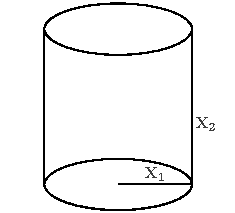
\includegraphics{kepek/kkthenger.pdf}
\end{multicols}

\begin{megoldas}
A KKT feltételek felírásához csoportosítjuk és egyszerűsítjük a feltételeket:
\begin{alignat*}{2}
f&:x_1^2+x_1x_2\\
g_1&:16-x_1^2x_2
\end{alignat*}
\end{megoldas}

\begin{megoldas}
A Lagrange függvény és gradiensei ekkor a következőek:
\begin{gather*}
L(x_1,x_2,u_1)=f+u_1\cdot g_1=x_1^2+x_1x_2+u_1(16-x_1^2x_2)\\
\nabla L=\left(\begin{array}{c}2x_1+x_2-2x_1x_2u_1\\x_1-x_1^2u_1\\\hdashline16-x_1^2x_2\end{array}\right)\quad H=\nabla^2L=\left(\begin{array}{cc:c}2-2x_2u_1&1-2x_1x_2&-2x_1x_2\\1-2x_1x_2&0&-x_1^2\\\hdashline-2x_1x_2&-x_1^2&0\end{array}\right)
\end{gather*}

A KKT feltételek ebből kiolvasva:
\begin{alignat*}{2}
\left.\begin{aligned}
        2x_1+x_2-2x_1x_2u_1&=0\\
        x_1-x_1^2u_1&=0
      \end{aligned}
\right\} &\mbox{ duál feltételek}\\
\left.
        u_1(16-x_1^2x_2)=0
\right.\hskip 0.24cm &\mbox{ komplementaritási feltétel}\\
\left.\begin{aligned}
        16-x_1^2x_2&\leq 0\\
        u_1&\geq 0
      \end{aligned}
\right\} &\mbox{ primál feltételek}
\end{alignat*}

Ezután esetszétválasztással megkeressük az összes KKT pontot:

\textbf{I. eset}: $u_1=0$
\begin{alignat*}{2}
2x_1+x_2&=0\\
x_1&=0\\
16-x_1^2x_2&\leq0
\end{alignat*}

Ebből egyszerűen adódik, hogy $\mathbf{x}=(0,0)^T$, azonban ez nem KKT pont, mert $16\not\leq 0$. Szemléletesen pedig nyilvánvaló hogy egy zérus átmérőjű és magasságú henger térfogata nem lesz megfelelő.

\textbf{II. eset}: $u_1>0$
\begin{alignat*}{2}
2x_1+x_2-2x_1x_2u_1&=0\\
x_1(1-x_1u_1)&=0\\
16-x_1^2x_2&=0
\end{alignat*}

A második feltételnél szétválasztjuk az esetet:

\indent\indent\textbf{II/a. eset}: $x_1=0$. Ekkor $x_2=0$-t kapunk, de azt már beláttuk hogy en nem KKT pont.

\indent\indent\textbf{II/b. eset}: $x_1u_1=1$
\begin{alignat*}{2}
2x_1+x_2-2x_2=&0 \mbox{ azaz } x_2=2x_1\\
16-x_1^2x_2=0
\end{alignat*}
\indent Ebből egyszerűen kijön, hogy
\begin{alignat*}{2}
16&=2x_1^3\\
x_1^3&=8\\
x_1&=2\\
x_2&=4
\end{alignat*}

Az $u_1$ Lagrange szorzó értéke ekkor $\nicefrac{1}{2}$. Az $\mathbf{x}=(2,4)^T$ pont KKT pont, hiszen teljesíti az összes feltételt. Azonban, hogy optimális megoldás legyen teljesülnie kell annak, hogy $H(\textbf{x})$ pozitív definit mátrix legyen.
\end{megoldas}

\begin{megoldas}
A Hesse-féle mátrix értéke az $\mathbf{x}=(2,4)^T$ helyen ($u_1=\nicefrac{1}{2}$):
\begin{gather*}
H(\mathbf{x})=\nabla^2f(\mathbf{x})=\begin{pmatrix}-2&-1&-16\\-1&0&-4\\-16&-4&0\end{pmatrix}
\end{gather*}

Az inerciateszttel ellenőrízhetjük a definitségét:
\begin{gather*}
\underbrace{\left|\begin{array}{ccc}\circled{-2}&-1&-16\\-1&0&-4\\-16&-4&0\end{array}\right|}_\text{Iner(1,0,0)}\sim
\underbrace{\left|\begin{array}{cc}\nicefrac{1}{2}&4\\4&\circled{128}\end{array}\right|}_\text{Iner(0,0,1)}\sim\underbrace{\left|\begin{array}{c}\nicefrac{3}{8}\end{array}\right|}_\text{Iner(0,0,1)}
\end{gather*}

Ez alapján az inercia értéke $\mbox{Iner}(1,0,2)$, tehát H feltételesen pozitív definit mátrix, ezért a $\mathbf{x}=(2,4)^T$ pont valóban optimális minimumpont.
\end{megoldas}


\feladatszam Adott az $x_2^2=x_1+3$ parabola. A parabola az $(x_1,x_2)$ síkot két tartományra osztja. Tekintse azt a tartományt, amely az origót tartalmazza. Határozza meg a tartomány azon pontjait, amelyeknél az $f(x_1,x_2)=x_1x_2$ függvény értéke a legkisebb! A megoldást az alábbi lépésekben végezze el:
\begin{alphanumericlist}
\item Írja fel az optimalizációs feladatot matematikai formában!
\item Határozza meg az összes KKT pontot!
\item Döntse el, hogy az egyes KKT pontok közül melyik lokális minimumpont!
\item Határozza meg a globális minimumpontot!
\end{alphanumericlist}

\begin{megoldas}
Először is célszerű készíteni egy ábrát a paraboláról.
\begin{center}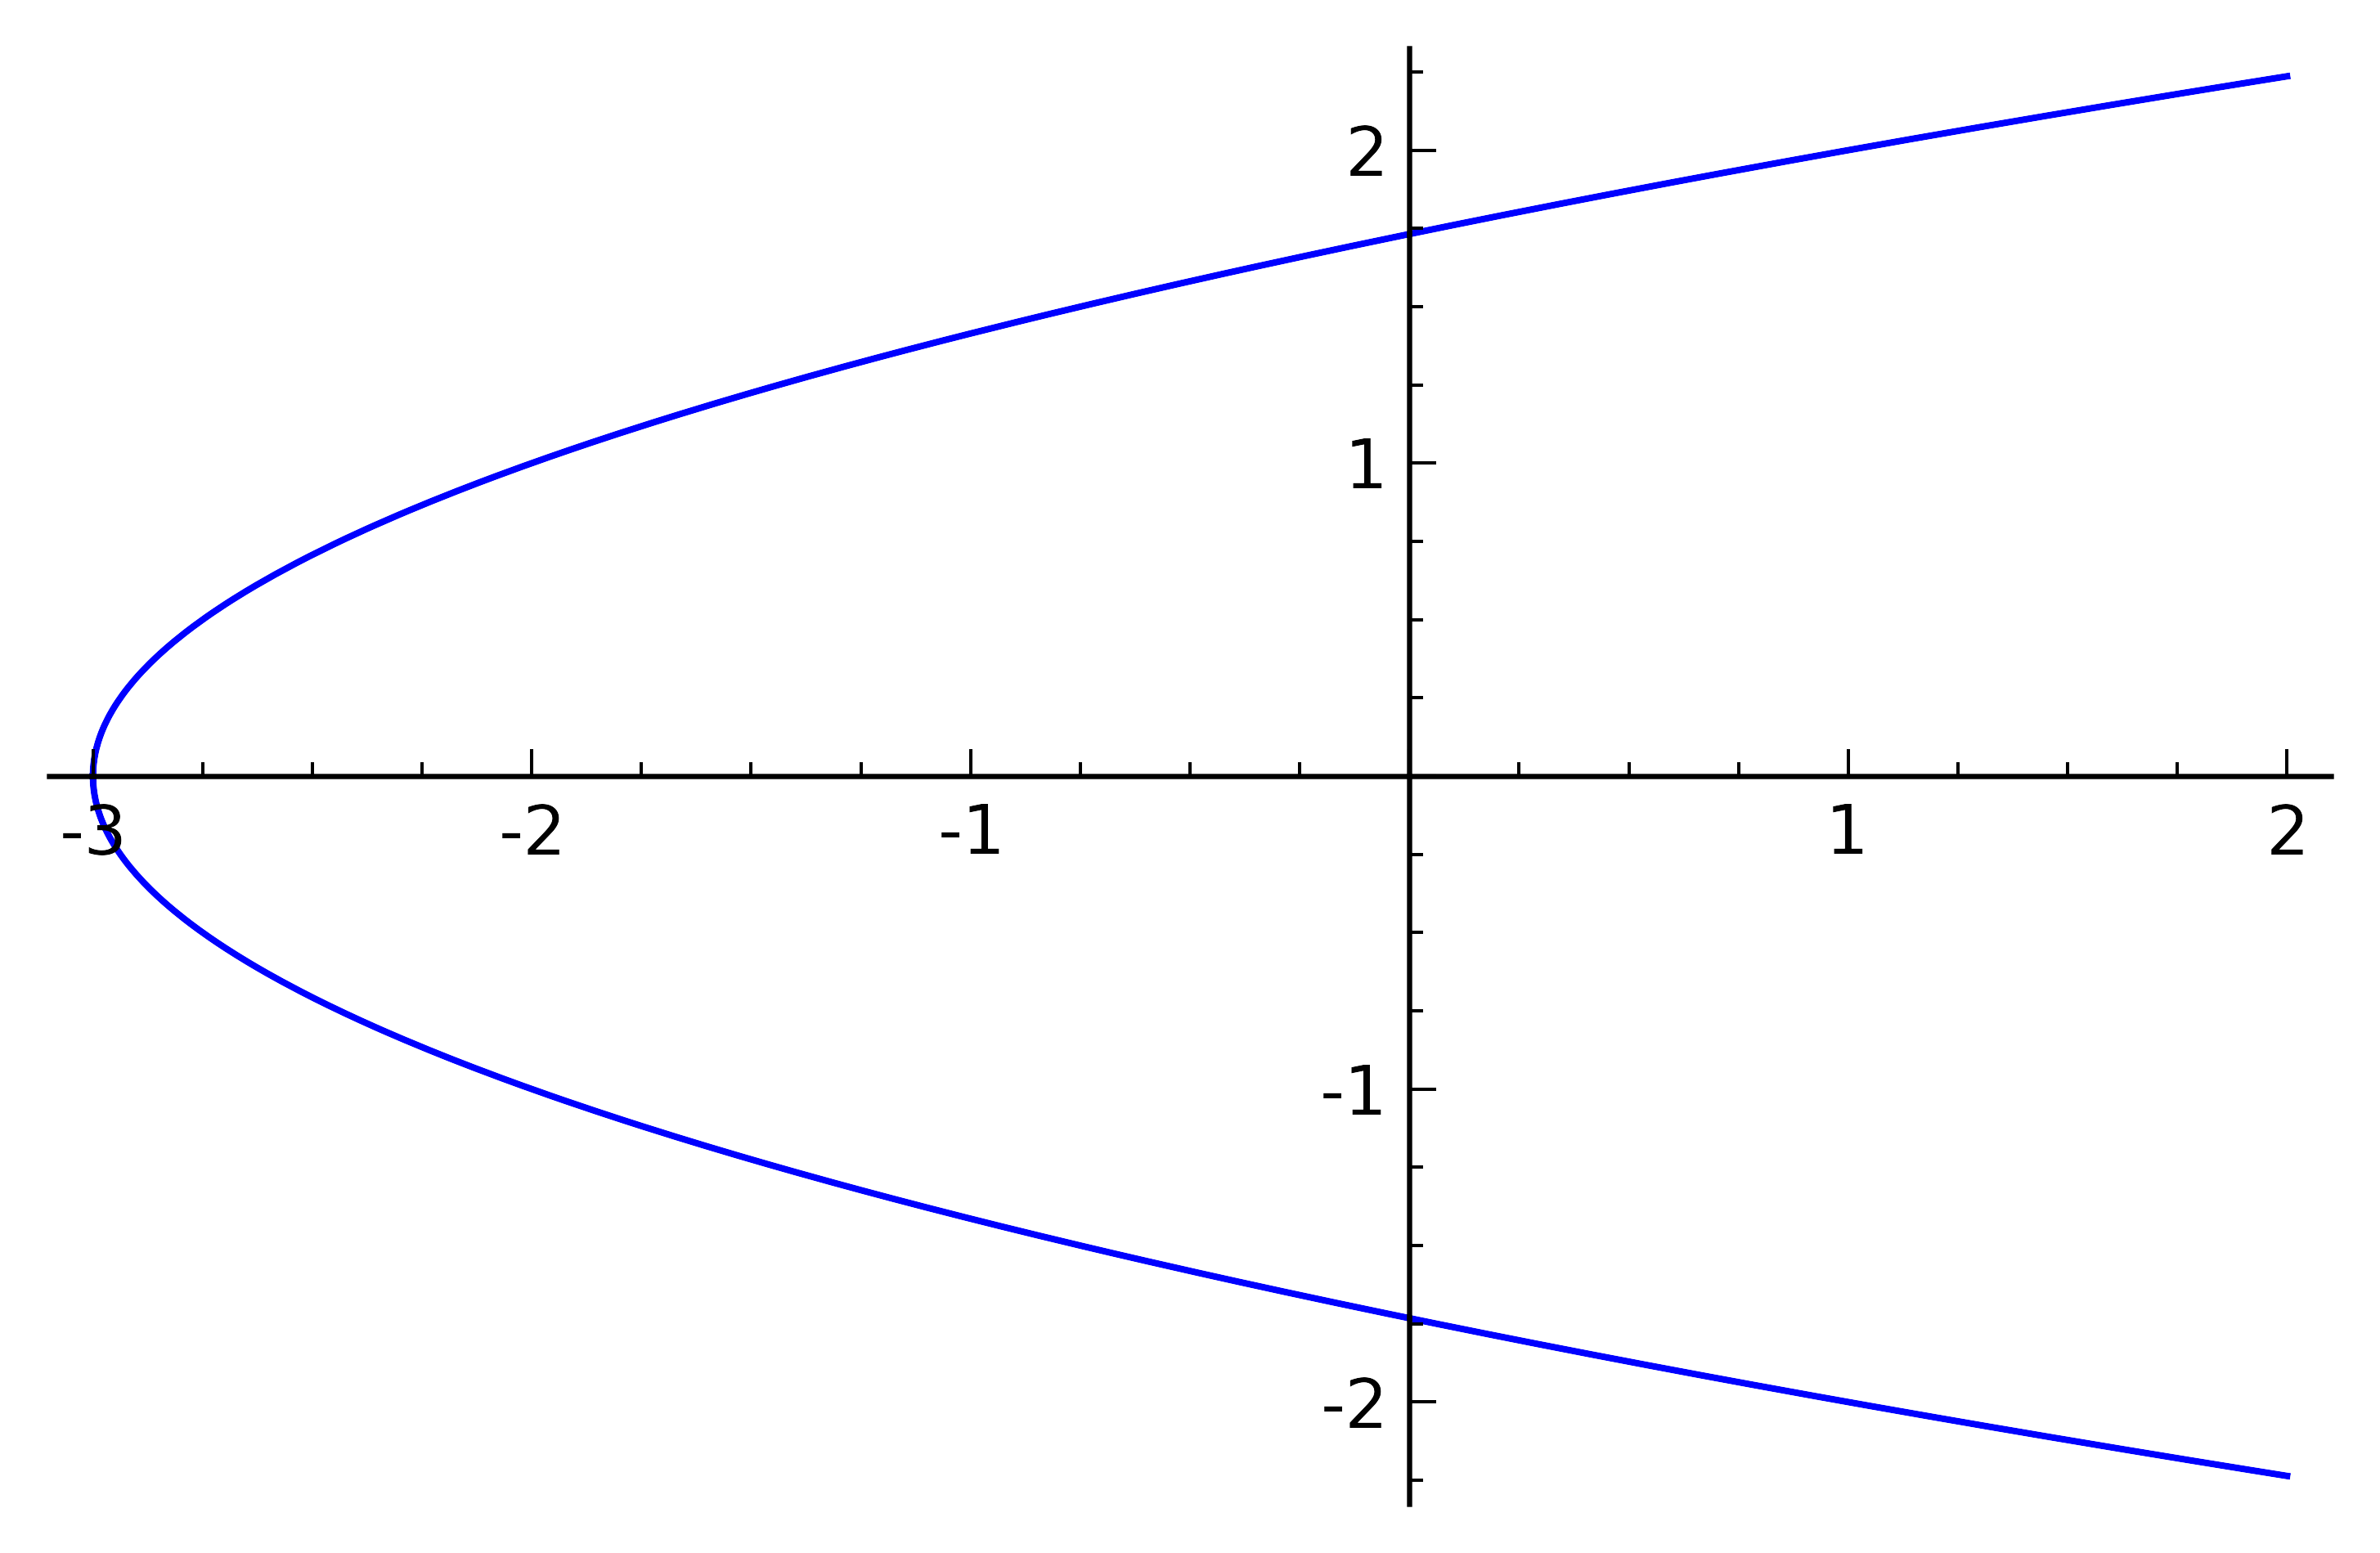
\includegraphics[scale=0.65]{kepek/kktparabola.png}\end{center}

A feladat matematikailag megfogalmazva a következő:
\begin{alignat*}{2}
x_2^2-x_1-3\leq0\\
x_1x_2\longrightarrow\min!
\end{alignat*}
\end{megoldas}

\begin{megoldas}
Most már kiszámolhatjuk a Lagrange függvényt és gradienseit:
\begin{gather*}
L(x_1,x_2,u_1,u_2)=x_1x_2+u_1(x_2^2-x_1-3)\\
\nabla L=\left(\begin{array}{c}x_2-u_1\\x_1+2x_2u_1\\\hdashline x_2^2-x_1-3\end{array}\right)\quad H=\nabla^2L=\left(\begin{array}{cc:c}0&1&-1\\1&2u_1&2x_2\\\hdashline-1&2x_2&0\end{array}\right)
\end{gather*}

A KKT feltételeket kiolvasva:
\begin{alignat*}{2}
    \left.\begin{aligned}
      x_2-u_1&=0\\
      x_1+2x_2u_1&=0
    \end{aligned}\right\} &\mbox{ duális feltételek}\\
u_1(x_2^2-x_1-3)=0\hskip 0.27cm &\mbox{ komplementaritási feltétel}\\
    \left.\begin{aligned}
      x_2^2-x_1-3&\leq0\\
      u_1&\geq0
    \end{aligned}\right\} &\mbox{ primál feltételek} 
\end{alignat*}

Esetszétválasztás:

\textbf{I. eset}: $u_1=0$
\begin{alignat*}{2}
x_2&=0\\
x_1&=0
\end{alignat*}

Ez teljesíti is a KKT feltételeket (azaz KKT pont), nézzük meg a H definitását!
\begin{gather*}
\underbrace{
\left|\begin{array}{ccc}0&\circled{1}&-1\\1&0&0\\-1&0&0\end{array}\right|\sim
\left|\begin{array}{cc}\circled{1}&0\\-1&0\end{array}\right|}_\text{Iner(1,0,1)}
\sim\underbrace{\left|\begin{array}{c}0\end{array}\right|}_\text{Iner(0,1,0)}
\end{gather*}

Az inercia értéke $\mbox{Iner}(1,1,1)$, tehát a mátrix indefinit, így az $\mathbf{x}=(0,0)^T$ csak nyeregpont.

\textbf{II. eset}: $u_1>0$
\begin{alignat*}{2}
x_2&=u_1\\
x_1+2x_2u_1&=0\\
x_2^2-x_1-3&=0
\end{alignat*}

A második egyenletbe az elsőt behelyettesítve: $x_1=-2u_1^2$. Ezt és az első egyenletet a harmadikba behelyettesítve: $u_1^2+2u_1^2-3=0$ azaz $u_1^2=1$. Ez tehát két megoldást is szolgáltat:
\begin{alignat*}{4}
u_1&=1&\quad&u_1&=-1\\
x_1&=-2&&x_1&=-2\\
x_2&=1&&x_2&=-1
\end{alignat*}

Mindkettő KKT pontot szolgáltat, a Hesse-féle mátrix definitségét vizsgálni kell:
\end{megoldas}

\begin{megoldas}
\begin{gather*}
\underbrace{\left|\begin{array}{ccc}0&1&-1\\1&\circled{$2$}&2\\-1&2&0\end{array}\right|}_\text{Iner(0,0,1)}\sim
\underbrace{\left|\begin{array}{cc}\circled{$-\nicefrac{1}{2}$}&-2\\-2&-2\end{array}\right|}_\text{Iner(1,0,0)}
\sim\underbrace{\left|\begin{array}{c}6\end{array}\right|}_\text{Iner(0,0,1)}\\
\underbrace{\left|\begin{array}{ccc}0&1&-1\\1&\circled{$-2$}&-2\\-1&-2&0\end{array}\right|}_\text{Iner(1,0,0)}\sim
\underbrace{\left|\begin{array}{cc}\circled{$\nicefrac{1}{2}$}&-2\\-2&-2\end{array}\right|}_\text{Iner(0,0,1)}
\sim\underbrace{\left|\begin{array}{c}-10\end{array}\right|}_\text{Iner(1,0,0)}
\end{gather*}

Az $\mathbf{x}=(-2,1)^T$ KKT ponthoz tartozó Hesse-féle mátrix feltételesen pozitív definit, míg az $\mathbf{x}=(-2,-1)^T$ KKT ponthoz tartozó feltételesen negatív definit. Tehát az első pont lokális minimum, a második pedig lokális maximum pont. A következő kontúrrajzon ez jól látszik:
\begin{center}
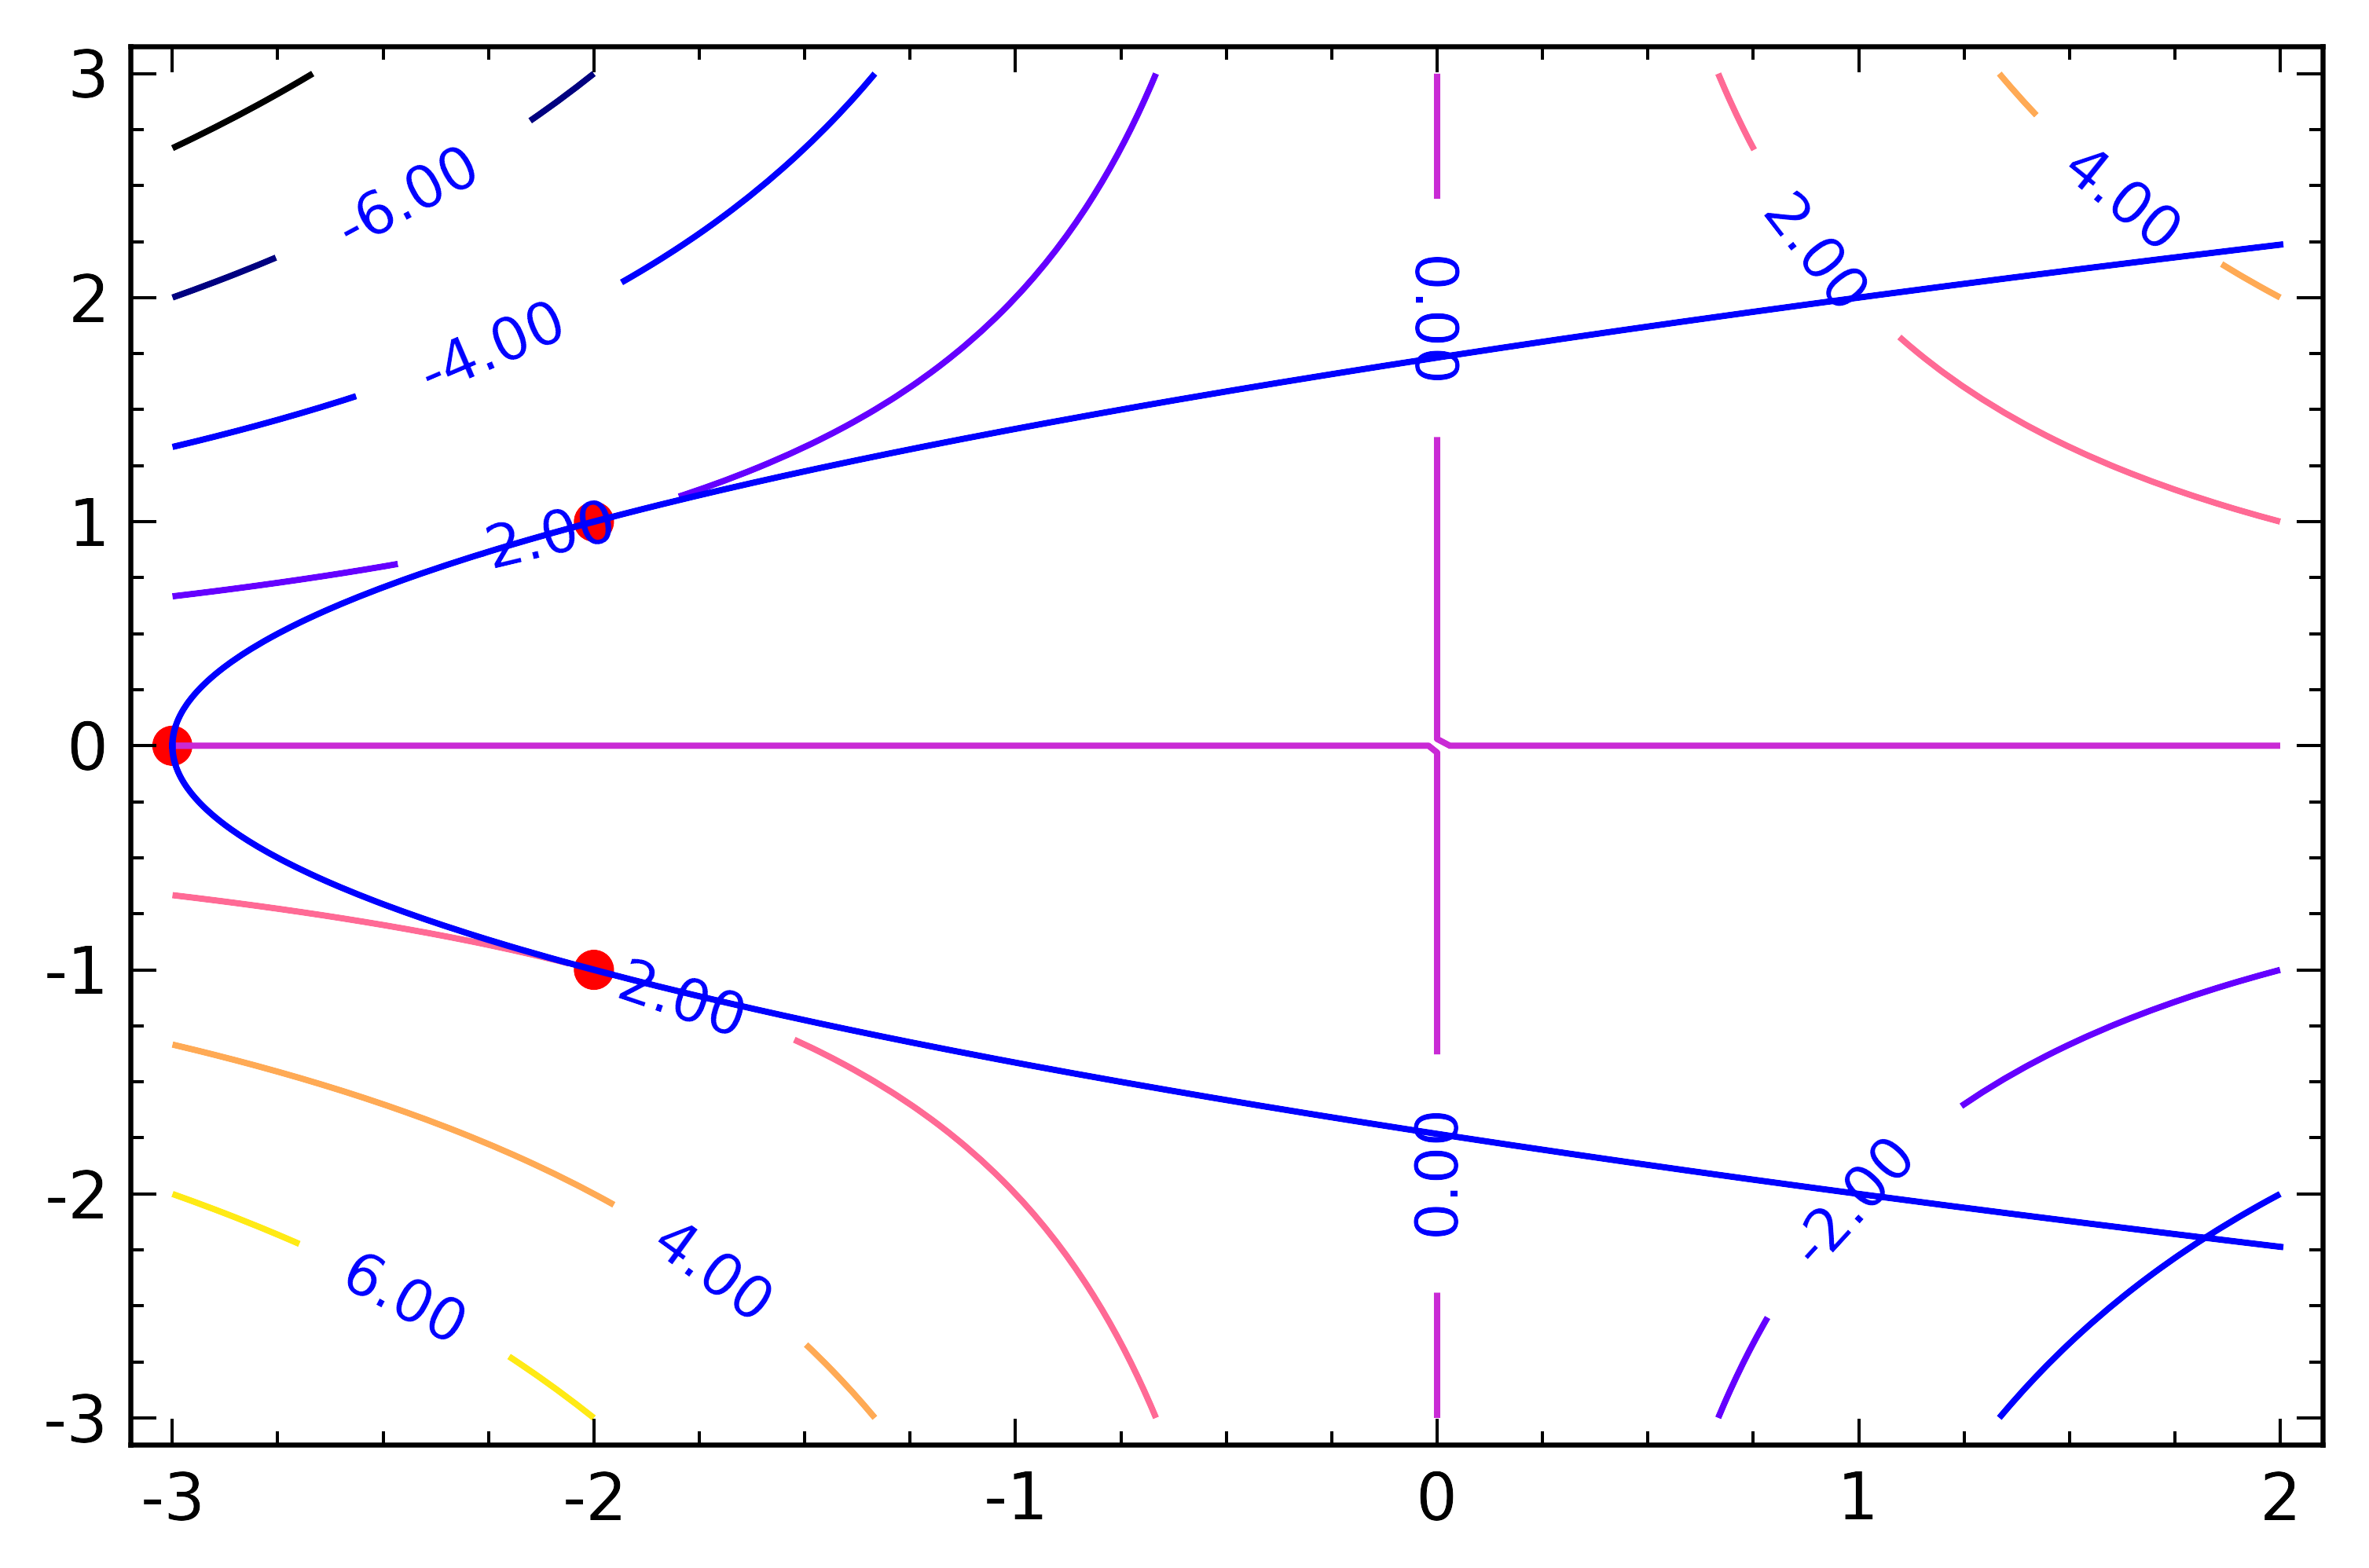
\includegraphics[scale=1]{kepek/kktkontur.png}
\end{center}

Globális minimuma pedig nem létezik a függvénynek, hiszen az $x_1$ tetszőlegesen nagy pozitív számnak, az $x_2$ pedig tetszőlegesen kicsi negatív számnak választható (természetesen csak a tartományon belül maradva), így az $f(x_1,x_2)=x_1x_2$ célfüggvény tetszőlegesen kis értéket vehet fel.
\end{megoldas}


\section{Extrémum keresés}

\firstline A következő keresési módszerek úgy működnek, hogy veszünk egy keresési intervallumot, amelyet különböző módokon felosztunk, majd megnézzük hogy melyik részében szerepel az optimum. Ezt rekurzívan folytatjuk a leállási feltétel teljesüléséig.

A felosztás mindig két részre bontja az intervallumot az alábbi módon:
\begin{center}
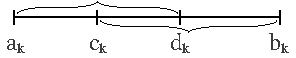
\includegraphics{kepek/extremum.pdf}
\end{center}

A megfelelő intervallum kiválasztása, és a következő $a$ és $b$ paraméterek kiválasztása az alábbi módon történik:
\begin{alignat*}{3}
\mbox{Ha } f(c_k)&<f(d_k) &\qquad \mbox{Ha } f(c_k)&\geq f(d_k)\\
a_{k+1}&=a_k & a_{k+1}&=c_k\\
b_{k+1}&=d_k & b_{k+1}&=b_k 
\end{alignat*}

\subsection{Dichotomous-módszer}

\firstline A módszer során az intervallumok meghatározásához egy $\delta$ paramétert alkalmazunk, amelyet előre kiválasztunk. A keresés addig tart, amíg az intervallum hossza nagyobb, mint a megadott $\varepsilon$ paraméter.
\begin{gather*}
c_k=a_k+\frac{L_k}{2}-\delta \qquad
d_k=a_k+\frac{L_k}{2}+\delta 
\end{gather*}

\subsection{Aranymetszés (Golden Section) módszer}

\firstline A módszernél a keresési intervallumot az aranymetszés arányában osztjuk fel:
\begin{gather*}
c_k=a_k+(1-\varphi)L_k \qquad
d_k=a_k+\varphi L_k
\end{gather*}

ahol $\varphi=\tfrac{\sqrt{5}-1}{2}$. A keresés szintén addig tart, amíg $L_k>\varepsilon$.

\subsection{Fibonacci-módszer}

\firstline A Fibonacci módszer esetén a Fibonacci-számok segítségével határozzuk meg az intervallumokat. A Fibonacci-számokat az alábbiak szerint definiáljuk:
\begin{gather*}
F_n=\begin{cases}
    0,&\mbox{ha } n=0\\[-0.3em]
    1,&\mbox{ha } n=1\\[-0.3em]
    F_{n-1}+F_{n-2},&\mbox{ha } n\geq2
\end{cases}
\end{gather*}

Az intervallumok meghatározása pedig:
\begin{gather*}
c_k=a_k+\frac{F_{n-k-1}}{F_{n-k+1}}L_k \qquad
d_k=a_k+\frac{F_{n-k}}{F_{n-k+1}}L_k 
\end{gather*}

A módszer használatához választunk egy kezdeti $n$ paramétert, amely meghatározza a pontosságot.

\subsection{Példafeladat}

\feladatszam Adott az $f(x)=x^2-4x+3\longrightarrow\min!$ optimalizálási feladat. Adott továbbá az $[a_1,b_1]=[1,3]$ bizonytalansági intervallum.
\begin{alphanumericlist}
\item Határozza meg az $[a_2,b_2]$ bizonytalansági intervallumot:
  \begin{itemize}
    \item Dichotomous módszerrel $\delta =0,3$ paraméter esetén
    \item Aranymetszés módszerrel
    \item Fibonacci módszerrel $n=8$ paraméter esetén
  \end{itemize}
\item Határozza meg aranymetszés módszer esetén az $[a_6,b_6]$ bizonytalansági intervallum hosszát!
\end{alphanumericlist}

\begin{megoldas}
Az intervallum hossza $L_1=3-1=2$. A Dichotomous módszer esetén
\begin{alignat*}{4}
c_1=a_1+\frac{L_1}{2}-\delta&=1+\frac{2}{2}-0,3=1,7 &\qquad d_1=a_1+\frac{L_1}{2}+\delta&=1+\frac{2}{2}-0,3=2,3\\
f(c_1)&=-0,91 & f(d_1)&=-0,91
\end{alignat*}

Mivel $f(c_1)\geq f(d_1)$, ezért $a_2=c_1=1,7$, és $b_2=b_1=3$.

Az aranymetszés módszer esetén:
\begin{alignat*}{4}
c_1=a_1+(1-\varphi)L_1&=1+0,38197\cdot2=1,7639&\qquad d_1=a_1+\varphi L_1&=1+0,6180\cdot2=2,2361\\
f(c_1)&=-0,9443&f(d_1)&=-0,9443
\end{alignat*}

Mivel $f(c_1)\geq f(d_1)$, ezért $a_2=c_1=1,7639$, és $b_2=b_1=3$.

A Fibonacci módszer esetén:
\begin{alignat*}{4}
c_1=a_1+\frac{F_6}{F_8}L_1&=1+\frac{8}{21}\cdot2=1,7619&\qquad d_1=a_1+\frac{F_7}{F_8}L_1&=1+\frac{13}{21}\cdot2=2,2381\\
f(c_1)&=-0,9433&f(d_1)&=-0,9433
\end{alignat*}

Mivel $f(c_1)\geq f(d_1)$, ezért $a_2=c_1=1,7619$, és $b_2=b_1=3$.

\medskip\hrule\medskip

Az $[a_6,b_6]$ intervallum hossza $L_1\cdot\varphi^5=0,1803$.

\end{megoldas}

\section{Gradiens-módszer}

\subsection{Konjugált gradiens módszer}

\firstline Választunk egy $x_0$ kezdőpontot, ahonnan elindulunk. A kezdeti $d_0$ irány a szokásos módon $d_0=-\nabla f(x_0)$. Az ezt követő elemeket az alábbiakból kaphatjuk:
\begin{align*}
x_{k+1}&=x_k+\lambda d_k\\
d_k&=-\nabla f(x_{k+1})+\alpha_{k+1}d_k\\
\alpha_{k+1}&=\frac{||\nabla f(x_{k+1})||_2^2}{||\nabla f(x_{k})||_2^2}
\end{align*}

Másképp megfogalmazva, a gradiensek elemeinek a négyzetösszegét osztjuk el egymással. Az $x_{k+1}$ pont meghatározásához szükséges $\lambda$-t a következő módon kaphatjuk meg:

\begin{numericlist}
\item Az $x_k+\lambda d_k$ vektort behelyettesítjük az $f$ függvénybe. Ezt $\phi(\lambda)$-val jelöljük.
\item A $\phi'(\lambda)=0$ megoldásai közül kerülhet ki a $\lambda$ értéke, hiszen itt lehet lokális minimuma a függvénynek. Ha egyetlen $\lambda$ érték jöhet szóba, akkor azt választjuk.
\item Az eljárás addig tart amíg $\lambda$ nullától különböző vagy egy megadott értéknél abszolútértékben nagyobb.
\end{numericlist}

\subsection{Példafeladatok}

\feladatszam Az alábbi függvény minimumát szeretnénk meghatározni konjugált gradiens módszerrel:
\begin{align*}
f(x_1,x_2)=x_1^2+x_2^2+x_1-2x_2+7
\end{align*}

Tegyük fel, hogy már néhány lépést elvégeztünk, és alábbi eredményeket kaptuk:
\begin{align*}
x_6=\left(\begin{array}{c}0\\1+\frac{\sqrt{2}}{3}\end{array}\right) \quad 
d_6=\left(\begin{array}{c}\frac{1}{2}\\\frac{1}{2}\end{array}\right) \quad
x_7=\left(\begin{array}{c}\frac{1}{2}\\4\end{array}\right)
\end{align*}

Határozza meg az $x_8$ közelítést, és a hozzá tartozó $d_7$ vektort!

\begin{megoldas}
Az irányvektort meghatározhatjuk a megadott adatokból, csak a gradiens értékére van szükségünk hozzá:
$$d_7=-\nabla f(x_7)+\frac{||\nabla f(x_{7})||_2^2}{||\nabla f(x_6)||_2^2}d_6$$
$$\nabla f(x_1,x_2)=\left(\begin{array}{c}2x_1+1\\2x_2-2\end{array}\right)$$

A behelyettesítés után:
\begin{align*}d_7=-\left(\begin{array}{c}2\\[0.3em]6\end{array}\right)+\frac{2^2+6^2}{2^2+(-1)^2}\left(\begin{array}{c}\frac{1}{2}\\[0.3em]\frac{1}{2}\end{array}\right)= \left(\begin{array}{c}-2\\[0.3em]-6\end{array}\right)+10\left(\begin{array}{c}\frac{1}{2}\\[0.3em]\frac{1}{2}\end{array}\right)=\left(\begin{array}{c}3\\[0.3em]-1\end{array}\right)\end{align*}

Ezt felhasználva, most már meg tudjuk mondani $x_8$ értékét:
\begin{align*}x_8=x_7+\lambda d_7=\left(\begin{array}{c}\frac{1}{2}+3\lambda\\[0.3em]4-\lambda\end{array}\right)\end{align*}

A $\lambda$ értékének meghatározásához behelyettesítünk:
\begin{align*}
\varphi(\lambda)&=(\tfrac{1}{2}+3\lambda)^2+(4-\lambda)^2+(\tfrac{1}{2}+3\lambda)-2(4-\lambda)+7\\
\varphi'(\lambda)&=18\lambda+3+2\lambda-8+3+2=20\lambda = 0 \longrightarrow \lambda=0
\end{align*}

Tehát $x_8$ megegyezik $x_7$-tel, így az algoritmus meg is állna.
\end{megoldas}


\feladatszam Oldja meg az alábbi optimalizálási feladatot konjugált gradiens módszerrel, ha az első öt lépés utáni eredmények az alábbiak: 
\begin{gather*}
x_5 = \left(\begin{array}{c}0\\0\end{array}\right) \quad 
x_6 = \left(\begin{array}{c}1\\-1\end{array}\right) \quad
d_5 = \left(\begin{array}{c}1\\-1\end{array}\right)\\
f(x_1,x_2)=x_1^2+3x_1x_2+2x_2^2-x_1+x_2+3\rightarrow\min!
\end{gather*}


\begin{megoldas}
\begin{gather*}
\nabla f(x_1,x_2)=\left(\begin{array}{c}2x_1+3x_2-1\\2x_2+3x_1+1\end{array}\right)\\
d_6=-\nabla f(x_6)+\frac{||\nabla f(x_{6})||_2^2}{||\nabla f(x_5)||_2^2}d_5=-\left(\begin{array}{c}-2\\2\end{array}\right)+\frac{(-2)^2+2^2}{(-1)^2+1^2}\left(\begin{array}{c}1\\-1\end{array}\right)=\left(\begin{array}{c}6\\-6\end{array}\right)\\
x_7=x_6+\lambda d_6=\left(\begin{array}{c}1\\-1\end{array}\right)+\lambda\left(\begin{array}{c}6\\-6\end{array}\right)=\left(\begin{array}{c}1+6\lambda\\-1-6\lambda\end{array}\right)
\end{gather*}

A $\lambda$ behelyettesítése után:
\begin{alignat*}{1}
\varphi(\lambda)&=(1+6\lambda)^2-3(1+6\lambda)^2+2(1+6\lambda^2)-(1+6\lambda)-(1+6\lambda)+3\\
&=-2(1+6\lambda)+3=-12\lambda+1\\
\varphi'(\lambda)&=-12\neq0
\end{alignat*}

A $\lambda$ értéke nem határozható meg, ezért az algoritmus megáll.
\end{megoldas}


\section{Newton és kvázi Newton módszerek}

\subsection{Newton-módszer}

\subsection{Broyden--Fletcher--Goldfarb--Shanno (BFGS) módszer}

$$B_{k+1}=B_k+\frac{y_ky_k^T}{y_k^Ts_k}-\frac{(B_ks_k)(B_ks_k)^T}{(B_ks_k)^Ts_k}$$

A képletben az $s_k$ vektor az $B_ks_k=-\nabla f(x^{(k)})$ lineáris egyenletrendszer megoldása, az $y_k$ pedig az $\nabla f(x^{(k+1)})-\nabla f(x^{(k)})$ különbség.

\subsection{Davidon--Fletcher--Powell (DFP) módszer}

$$D_{k+1}=D_k+\frac{s_ks_k^T}{s_k^Ty_k}-\frac{(D_ky_k)(D_ky_k)^T}{(D_ky_k)^Ty_k}$$

A képletben az $s_k$ vektor az $-D_k\cdot\nabla f(x^{(k)})$ kifejezés értéke, az $y_k$ pedig az $\nabla f(x^{(k+1)})-\nabla f(x^{(k)})$ különbség.

\subsection{Példafeladatok}

\feladatszam Adott az $x_1^2+\nicefrac{1}{2}x_2^2\longrightarrow\min!$ optimalizási feladat. Adott továbbá egy $\mathbf{x}_5=\left(\begin{smallmatrix}1\\-1\end{smallmatrix}\right)$ közelítő vektor és a Hesse-féle mátrixot helyettesítő $\left(\begin{smallmatrix}2&-1\\-1&4\end{smallmatrix}\right)$ mátrix. A megoldást kvázi-Newton módszerrel kívánjuk meghatározni.
\begin{alphanumericlist}
\item Határozza meg az $\mathbf{x}_6$ közelítő megoldásvektort és a Hesse mátrixot helyettesítő új mátrixot, ha nem alkalmaz vonalmenti keresést!
\item Határozza meg az $\mathbf{x}_6$ közelítő megoldásvektort ha alkalmaz vonalmenti keresést! A Hesse mátrixot helyettesítő új mátrixot nem kell meghatározni, csak a kiszámításához szükséges két vektort számolja ki!
\end{alphanumericlist}

\begin{megoldas}
A feladat megoldható mind DFP, mind BFGS módszerrel. Mindkét módszerhez szükségünk van a $f$ függvény gradiensére, így előszer ezt számoljuk ki:
\begin{gather*}
\nabla f=\left(\begin{array}{c}2x_1\\x_2\end{array}\right)
\end{gather*}

A módszerek közül először tekintsük a DFP módszert! Ekkor a következő egyenletet kell megoldanunk:
\begin{alignat*}{1}
s_5&=-D_5\cdot\nabla f(\mathbf{x}_5)\\
s_5&=-\left(\begin{array}{cc}2&-1\\-1&4\end{array}\right)\cdot\left(\begin{array}{c}2\\-1\end{array}\right)\\
s_5&=\left(\begin{array}{c}-5\\6\end{array}\right)
\end{alignat*}

A $D_6$ mátrix kiszámításához az alábbi képletbe kell behelyettesítenünk:
\begin{gather*}
D_6=D_5+\frac{s_5s_5^T}{s_5^Ty_5}-\frac{(D_5y_5)(D_5y_5)^T}{(D_5y_5)^Ty_5}
\end{gather*}

Az $s_5$-öt már kiszámoltuk, az $y_5$ értéke pedig $\nabla f(\mathbf{x}_6)-\nabla f(\mathbf{x}_5)=\nabla f(\mathbf{x}_5+s_5)-\nabla f(\mathbf{x}_5)=\left(\begin{smallmatrix}12\\-7\end{smallmatrix}\right)-\left(\begin{smallmatrix}2\\-1\end{smallmatrix}\right)=\left(\begin{smallmatrix}10\\-8\end{smallmatrix}\right)$. Így a következőt kell kiszámolni:
\begin{gather*}
D_6=\left(\begin{array}{cc}2&-1\\-1&4\end{array}\right)+
\frac{\overbracket[0.75pt]{\left(\begin{smallmatrix}-5\\6\end{smallmatrix}\right)
\cdot\left(\begin{smallmatrix}-5&6\end{smallmatrix}\right)}^{\left(\begin{smallmatrix}25&-30\\-30&36\end{smallmatrix}\right)}}
{\underbracket[.75pt]{\left(\begin{smallmatrix}-5&6\end{smallmatrix}\right)
\cdot\left(\begin{smallmatrix}10\\-8\end{smallmatrix}\right)}_{-98}}-
\frac{\overbracket[.75pt]{\left[\left(\begin{smallmatrix}2&-1\\-1&4\end{smallmatrix}\right)\cdot
\left(\begin{smallmatrix}10\\-8\end{smallmatrix}\right)\right]
\left[\left(\begin{smallmatrix}2&-1\\-1&4\end{smallmatrix}\right)\cdot
\left(\begin{smallmatrix}10\\-8\end{smallmatrix}\right)\right]^T}^{\left(\begin{smallmatrix}784&-1176\\-1176&1764\end{smallmatrix}\right)}
}{\underbracket[.75pt]{\left[\left(\begin{smallmatrix}2&-1\\-1&4\end{smallmatrix}\right)\cdot
\left(\begin{smallmatrix}10\\-8\end{smallmatrix}\right)\right]^T\cdot
\left(\begin{smallmatrix}10\\-8\end{smallmatrix}\right)}_{616}
}
\end{gather*}

A mátrix tehát a következő értékű:
\begin{gather*}
D_6=\left(\begin{array}{cc}2-\nicefrac{25}{98}-\nicefrac{784}{616}&-1+\nicefrac{30}{98}+\nicefrac{1176}{616}\\-1+\nicefrac{30}{98}+\nicefrac{1176}{616}&4-\nicefrac{36}{98}-\nicefrac{1764}{616}\end{array}\right)\approx\left(\begin{array}{cc}3,0176&1,2152\\1,2152&0,7690\end{array}\right)
\end{gather*}

Iránymenti keresés esetén annyi változik, hogy $\mathbf{x}_6=\mathbf{x}_5+\lambda d_5$-re, ahol $d_5=s_5$ (csak azért nevezzük át $d$-re, hogy jelezzük irányról van szó) és $\lambda$ értéke az $\varphi(\lambda)=f(1-5\lambda,-1+6\lambda)$ függvény minimuma.
\begin{alignat*}{1}
\varphi(\lambda)&=(1-5\lambda)^2+\tfrac{1}{2}(-1+6\lambda)^2\\
&=25\lambda^2-10\lambda+1+\tfrac{1}{2}(36\lambda^2-12\lambda+1)\\
&=43\lambda^2-16\lambda+\tfrac{3}{2}
\end{alignat*}
\end{megoldas}

\begin{megoldas}
A függvény minimuma ott található, ahol az első derivált értéke nulla:
\begin{alignat*}{1}
\varphi'(\lambda)&=0\\
86\lambda-16&=0\\
86\lambda&=16\\
\lambda&=\nicefrac{16}{86}
\end{alignat*}

Ebből tehát az $\mathbf{x}_6$ értéke $\left(\begin{smallmatrix}0,0698\\0,1163\end{smallmatrix}\right)$. A DFP módszer Hesse mátrixot helyettesítő mátrixához már csak az $y_5$-ra van szükségünk az pedig:
\begin{gather*}
y_5=\left(\begin{array}{c}2\cdot 0,0698-2\\0,1163+1\end{array}\right)=\left(\begin{array}{c}-2,1395\\1,1163\end{array}\right)
\end{gather*}

A BFGS módszer esetén a következő egyenletet kell megoldanunk:
\begin{alignat*}{1}
B_5s_5&=-\nabla f(\mathbf{x}_5)\\
\left(\begin{array}{cc}2&-1\\-1&4\end{array}\right)s_5&=\left(\begin{array}{c}-2\\1\end{array}\right)\\
s_5&=\left(\begin{array}{c}-1\\0\end{array}\right)
\end{alignat*}

A $B_6$ mátrix kiszámításához az alábbi képletbe kell behelyettesítenünk:
\begin{gather*}
B_6=B_5+\frac{y_5y_5^T}{y_5^Ts_5}-\frac{(B_5s_5)(B_5s_5)^T}{(B_5s_5)^Ts_5}
\end{gather*}
Az $s_5$-öt már kiszámoltuk, az $y_5$ értéke pedig $\nabla f(\mathbf{x}_6)-\nabla f(\mathbf{x}_5)=\nabla f(\mathbf{x}_5+s_5)-\nabla f(\mathbf{x}_5)=\left(\begin{smallmatrix}0\\-1\end{smallmatrix}\right)-\left(\begin{smallmatrix}2\\-1\end{smallmatrix}\right)=\left(\begin{smallmatrix}-2\\0\end{smallmatrix}\right)$. Így a következőt kell kiszámolni:
\begin{gather*}
D_6=\left(\begin{array}{cc}2&-1\\-1&4\end{array}\right)+
\frac{\overbracket[.75pt]{\left(\begin{smallmatrix}-2\\0\end{smallmatrix}\right)
\cdot\left(\begin{smallmatrix}-2&0\end{smallmatrix}\right)}^{\left(\begin{smallmatrix}4&0\\0&0\end{smallmatrix}\right)}}
{\underbracket[.75pt]{\left(\begin{smallmatrix}-2&0\end{smallmatrix}\right)
\cdot\left(\begin{smallmatrix}-1\\0\end{smallmatrix}\right)}_{2}}-
\frac{\overbracket[.75pt]{\left[\left(\begin{smallmatrix}2&-1\\-1&4\end{smallmatrix}\right)\cdot
\left(\begin{smallmatrix}-1\\0\end{smallmatrix}\right)\right]
\left[\left(\begin{smallmatrix}2&-1\\-1&4\end{smallmatrix}\right)\cdot
\left(\begin{smallmatrix}-1\\0\end{smallmatrix}\right)\right]^T}^{\left(\begin{smallmatrix}4&-2\\-2&1\end{smallmatrix}\right)}
}{\underbracket[.75pt]{\left[\left(\begin{smallmatrix}2&-1\\-1&4\end{smallmatrix}\right)\cdot
\left(\begin{smallmatrix}-1\\0\end{smallmatrix}\right)\right]^T\cdot
\left(\begin{smallmatrix}-1\\0\end{smallmatrix}\right)}_{2}
}\\
D_6=\left(\begin{array}{cc}2&0\\0&\nicefrac{7}{2}\end{array}\right)
\end{gather*}

Iránymenti keresés esetén $\mathbf{x}_6=\mathbf{x}+\lambda d_5$. A $\lambda$ meghatározásához a következő egyenlet minimumát keressük:
\begin{gather*}
\varphi(\lambda)=(1-\lambda)^2+\tfrac{1}{2}(-1)^2=\lambda^2-2\lambda+1+\tfrac{1}{2}=\lambda^2-2\lambda+\tfrac{3}{2}\\
\varphi'(\lambda)=0 \longrightarrow 2\lambda-2=0 \longrightarrow \lambda=1
\end{gather*}

Így tehát:
\begin{gather*}
y_5=\left(\begin{array}{c}-2\\0\end{array}\right)
\end{gather*}
Jelen esetben az iránymenti keresés nélküli módszer egybeesik az iránymenti keresésessel.
\end{megoldas}


\chapter{Hálózati folyamok}

\section{Szállítási feladat}

\feladatszam Három raktárban (R) 100, 120 és 120 tonnányi nyersanyagunk van. Az anyagot 5 felhasználó üzembe (Ü) kell szállítani, amelyek igénye rendre 40, 50, 70, 90 és 90 tonna. Az anyagok tonnánkénti szállítási költségét az alábbi táblázat tartalmazza. A feladatunk olyan szállítási terv készítése, mely minimális költséggel juttatja el a 240 tonna anyagot, feltéve hogy a szállítási költség arányos a szállított nyersanyag mennyiségével.
\begin{center}
\begin{tikzpicture}[
    covered/.style={decorate, draw=black, decoration={complete sines,amplitude=5pt, segment length=15pt}},
    cell/.style={nodes={rectangle,draw=black}},
    space/.style={matrix of nodes,row sep=-\pgflinewidth,column sep=-\pgflinewidth},
    text height = 3mm, anchor = center, text width = 7mm, nodes in empty cells,row sep=-\pgflinewidth,column sep=-\pgflinewidth,
]
    \matrix (magic) [matrix of nodes,
          nodes = {draw},
          text centered
    ]
    {%
        $1$ & $1$ & $2$ & $6$ & $9$\\
        $6$ & $4$ & $3$ & $5$ & $7$\\
        $5$ & $2$ & $6$ & $4$ & $8$\\
    };
    \node[text width = 1cm] at (-2.5,0.6) {$R_1$};
    \node[text width = 1cm] at (-2.5,0) {$R_2$};
    \node[text width = 1cm] at (-2.5,-0.6) {$R_3$};
    \node[text width = 1cm] at (-1.7,1.2) {$Ü_1$};
    \node[text width = 1cm] at (-0.7,1.2) {$Ü_2$};
    \node[text width = 1cm] at (0.3,1.2) {$Ü_3$};
    \node[text width = 1cm] at (1.25,1.2) {$Ü_4$};
    \node[text width = 1cm] at (2.2,1.2) {$Ü_5$};
\end{tikzpicture}
\end{center}

\begin{megoldas}
Mindenekelőtt vegyünk a költségmátrix sor-oszlopredukcióját:
\begin{center}
\begin{tikzpicture}[
    covered/.style={decorate, draw=black, decoration={complete sines,amplitude=5pt, segment length=15pt}},
    cell/.style={nodes={rectangle,draw=black}},
    space/.style={matrix of nodes,row sep=-\pgflinewidth,column sep=-\pgflinewidth},
    text height = 3mm, anchor = center, text width = 7mm, nodes in empty cells,row sep=-\pgflinewidth,column sep=-\pgflinewidth,
]
    \matrix (magic) [matrix of nodes,
          nodes = {draw},
          text centered
    ]
    {%
        $0$ & $0$ & $1$ & $3$ & $4$\\
        $0$ & $1$ & $0$ & $0$ & $0$\\
        $0$ & $0$ & $4$ & $0$ & $2$\\
    };
\end{tikzpicture}
\end{center}

Ez alapján jöhet az első lépés, melyben veszünk egy kezdeti szállítást (észak-nyugati sarok módszerrel), majd utat kersünk címkézéssel:
\begin{center}
\begin{tikzpicture}[
    covered/.style={decorate, draw=black, decoration={complete sines,amplitude=5pt, segment length=15pt}},
    cell/.style={nodes={rectangle,draw=black}},
    text height = 3mm, anchor = center, text width = 7mm, nodes in empty cells,row sep=-\pgflinewidth,column sep=-\pgflinewidth,
]
        \node[matrix] (magic_matrix) [matrix of nodes,
          nodes = {draw, anchor=center},
          text centered
        ] at (0,0)
    {%
        $40$ & $50$ & -- & -- & --\\
        $0$ & -- & $70$ & $50$ & $0$\\
        $0$ & $0$ & -- & $40$ & --\\
    };   
        \node[matrix] (magic_array_left) [matrix of nodes,
          nodes = {draw},
          text centered
        ] at (-3.3,0)
    {%
        $10$\\
        $0$\\
        $80$\\};   
        \node[matrix] (magic_array_top) [matrix of nodes,
          nodes = {draw},
          anchor=center,
          text centered
        ] at (0,1.5)
    {%
        $0$ & $0$ & $0$ & $0$ & $90$ \\
    };    
        \node[matrix] (magic_array_right) [matrix of nodes,
          nodes = {draw},
          text centered
        ] at (3.3,0)
    {%
        $+s$\\
        $+4$\\
        $+s$\\
    };    
        \node[matrix] (magic_array_bottom) [matrix of nodes,
          nodes = {draw},
          text centered
        ] at (0,-1.5)
    {%
        $+1$ & $+1$ & $-2$ & $+3$ & $-2$\\
    };
    
    \node[text width= 1.2cm] at (3.4, -1.5) {$\delta=50$};

    \draw[thick] (-3.6,-0.8) rectangle (-3,-0.4); 
    \draw[thick] (1,-0.6) circle(2.5mm);
    \draw[thick] (0.7,-0.2) rectangle (1.25,0.2);
    \draw[thick] (1.96,0) circle(2.5mm);
    \draw[thick] (1.65,1.3) rectangle (2.25,1.7);
    \draw[thick] (-3.0,-0.6) -- (0.75,-0.6);
    \draw[thick] (1,-0.35) -- (1,-0.2);
    \draw[thick] (1.25,0) -- (1.7,0);
    \draw[thick] (1.96,0.25) -- (1.96,1.3);
\end{tikzpicture}
\end{center}

Folytatjuk az útkeresést:
\begin{center}
\begin{tikzpicture}[
    covered/.style={decorate, draw=black, decoration={complete sines,amplitude=5pt, segment length=15pt}},
    cell/.style={nodes={rectangle,draw=black}},
    text height = 3mm, anchor = center, text width = 7mm, nodes in empty cells,row sep=-\pgflinewidth,column sep=-\pgflinewidth,
]
        \node[matrix] (magic_matrix) [matrix of nodes,
          nodes = {draw, anchor=center},
          text centered
        ] at (0,0)
    {%
        $40$ & $50$ & -- & -- & --\\
        $0$ & -- & $70$ & $0$ & $50$\\
        $0$ & $0$ & -- & $90$ & --\\
    };   
        \node[matrix] (magic_array_left) [matrix of nodes,
          nodes = {draw},
          text centered
        ] at (-3.3,0)
    {%
        $10$\\
        $0$\\
        $30$\\};   
        \node[matrix] (magic_array_top) [matrix of nodes,
          nodes = {draw},
          anchor=center,
          text centered
        ] at (0,1.5)
    {%
        $0$ & $0$ & $0$ & $0$ & $40$ \\
    };    
        \node[matrix] (magic_array_right) [matrix of nodes,
          nodes = {draw},
          text centered
        ] at (3.3,0)
    {%
        $+s$\\
        \\
        $+s$\\
    };    
        \node[matrix] (magic_array_bottom) [matrix of nodes,
          nodes = {draw},
          text centered
        ] at (0,-1.5)
    {%
        $+1$ & $+1$ & \phantom{$0$} & $+3$ & \phantom{$0$}\\
    };
\end{tikzpicture}
\end{center}

Mivel nem találtunk új utat, ezért lefedjük a sor-oszlop redukált táblát:
\begin{center}
\begin{tikzpicture}[
    covered/.style={decorate, draw=black, decoration={complete sines,amplitude=5pt, segment length=15pt}},
    cell/.style={nodes={rectangle,draw=black}},
    space/.style={matrix of nodes,row sep=-\pgflinewidth,column sep=-\pgflinewidth},
   text height = 3mm, anchor = center, text width = 7mm, nodes in empty cells,row sep=-\pgflinewidth,column sep=-\pgflinewidth,
]
        \matrix (magic) [matrix of nodes,
          nodes = {draw, anchor=center},
          text centered
        ]
    {%
        $0$ & $0$ & $1$ & $3$ & $4$\\
        $0$ & $1$ & $0$ & $0$ & $0$\\
        $0$ & $0$ & $4$ & $0$ & $2$\\
    };
    \draw[covered,thick] (magic-1-1.north) -- (magic-3-1.south);
    \draw[covered,thick] (magic-1-2.north) -- (magic-3-2.south);
    \draw[covered,thick] (magic-1-4.north) -- (magic-3-4.south);
    \draw[covered,thick] (magic-2-1.west) -- (magic-2-5.east);
\end{tikzpicture}
\end{center}

Az $\varepsilon$ értéke jelen esetben 1, frissítjük a táblát:
\begin{center}
\begin{tikzpicture}[
    covered/.style={decorate, draw=black, decoration={complete sines,amplitude=5pt, segment length=15pt}},
    cell/.style={nodes={rectangle,draw=black}},
    space/.style={matrix of nodes,row sep=-\pgflinewidth,column sep=-\pgflinewidth},
    text height = 3mm, anchor = center, text width = 7mm, nodes in empty cells,row sep=-\pgflinewidth,column sep=-\pgflinewidth,
]
        \matrix (magic) [matrix of nodes,
          nodes = {draw, anchor=center},
          text centered
        ]
    {%
        $0$ & $0$ & $0$ & $3$ & $3$\\
        $1$ & $2$ & $0$ & $1$ & $0$\\
        $0$ & $0$ & $3$ & $0$ & $1$\\
    };
\end{tikzpicture}
\end{center}
\end{megoldas}

\begin{megoldas}
Folytatjuk a keresést az új táblán:
\begin{center}
\begin{tikzpicture}[
    covered/.style={decorate, draw=black, decoration={complete sines,amplitude=5pt, segment length=15pt}},
    cell/.style={nodes={rectangle,draw=black}},
    text height = 3mm, anchor = center, text width = 7mm, nodes in empty cells,row sep=-\pgflinewidth,column sep=-\pgflinewidth,
]
        \node[matrix] (magic_matrix) [matrix of nodes,
          nodes = {draw, anchor=center},
          text centered
        ] at (0,0)
    {%
        $40$ & $50$ & $0$ & -- & --\\
        -- & -- & $70$ & -- & $50$\\
        $0$ & $0$ & -- & $90$ & --\\
    };   
        \node[matrix] (magic_array_left) [matrix of nodes,
          nodes = {draw},
          text centered
        ] at (-3.3,0)
    {%
        $10$\\
        $0$\\
        $30$\\};   
        \node[matrix] (magic_array_top) [matrix of nodes,
          nodes = {draw},
          anchor=center,
          text centered
        ] at (0,1.5)
    {%
        $0$ & $0$ & $0$ & $0$ & $40$ \\
    };    
        \node[matrix] (magic_array_right) [matrix of nodes,
          nodes = {draw},
          text centered
        ] at (3.3,0)
    {%
        $+s$\\
        $+3$\\
        $-s$\\
    };    
        \node[matrix] (magic_array_bottom) [matrix of nodes,
          nodes = {draw},
          text centered
        ] at (0,-1.5)
    {%
        $+1$ & $+1$ & $+1$ & $+3$ & $-2$\\
    };
    
    \node[text width= 1.2cm] at (3.4, -1.5) {$\delta=10$};

    \draw[thick] (-3.6,0.8) rectangle (-3,0.4); 
    \draw[thick] (0,0.6) circle(2.5mm);
    \draw[thick] (-0.25,-0.2) rectangle (0.25,0.2);
    \draw[thick] (1.96,0) circle(2.5mm);
    \draw[thick] (1.65,1.3) rectangle (2.25,1.7);
    \draw[thick] (-3.0,0.6) -- (-0.25,0.6);
    \draw[thick] (0,0.35) -- (0,0.2);
    \draw[thick] (0.25,0) -- (1.7,0);
    \draw[thick] (1.96,0.25) -- (1.96,1.3);
\end{tikzpicture}
\end{center}

Frissítjük a táblát, majd folytatjuk a keresést:
\begin{center}
\begin{tikzpicture}[
    covered/.style={decorate, draw=black, decoration={complete sines,amplitude=5pt, segment length=15pt}},
    cell/.style={nodes={rectangle,draw=black}},
    text height = 3mm, anchor = center, text width = 7mm, nodes in empty cells,row sep=-\pgflinewidth,column sep=-\pgflinewidth,
]
        \node[matrix] (magic_matrix) [matrix of nodes,
          nodes = {draw, anchor=center},
          text centered
        ] at (0,0)
    {%
        $40$ & $50$ & $10$ & -- & --\\
        -- & -- & $60$ & -- & $60$\\
        $0$ & $0$ & -- & $90$ & --\\
    };   
        \node[matrix] (magic_array_left) [matrix of nodes,
          nodes = {draw},
          text centered
        ] at (-3.3,0)
    {%
        $0$\\
        $0$\\
        $30$\\};   
        \node[matrix] (magic_array_top) [matrix of nodes,
          nodes = {draw},
          anchor=center,
          text centered
        ] at (0,1.5)
    {%
        $0$ & $0$ & $0$ & $0$ & $30$ \\
    };    
        \node[matrix] (magic_array_right) [matrix of nodes,
          nodes = {draw},
          text centered
        ] at (3.3,0)
    {%
        $+1$\\
        \phantom{$0$}\\
        $+s$\\
    };    
        \node[matrix] (magic_array_bottom) [matrix of nodes,
          nodes = {draw},
          text centered
        ] at (0,-1.5)
    {%
        $+3$ & $+3$ & $+1$ & $+3$ & $-3$\\
    };
    
    \node[text width= 1.2cm] at (3.4, -1.5) {$\delta=30$};

    \draw[thick] (-3.6,-0.8) rectangle (-3,-0.4); 
    \draw[thick] (-1.97,-0.6) circle(2.5mm);
    \draw[thick] (-2.25,0.4) rectangle (-1.7,0.8);
    \draw[thick] (0,0.6) circle(2.5mm);
    \draw[thick] (-0.25,-0.2) rectangle (0.25,0.2);
    \draw[thick] (1.96,0) circle(2.5mm);
    \draw[thick] (1.65,1.3) rectangle (2.25,1.7);
    
    \draw[thick] (-3,-0.6) -- (-2.22,-0.6);
    \draw[thick] (-1.97,0.4) -- (-1.97,-0.35);
    \draw[thick] (-1.7,0.6) -- (-0.25,0.6);
    \draw[thick] (0,0.35) -- (0,0.2);
    \draw[thick] (0.25,0) -- (1.7,0);
    \draw[thick] (1.96,0.25) -- (1.96,1.3);
\end{tikzpicture}
\end{center}

Ezzel megkaptuk az optimális megoldást.
\begin{figure}[H]
\centering
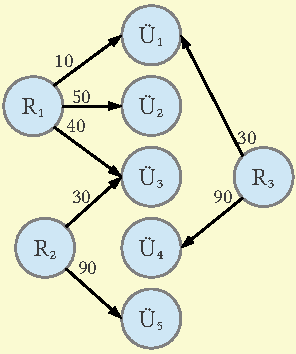
\includegraphics{kepek/szallitasi.pdf}
\end{figure}
A szállítás teljes költsége így 1400 pénzegység. 
\end{megoldas}

\section{Hozzárendelési feladat}

A hozzárendelési feladat tekinthető egy olyan szállítási feladatnak, ahol minden egyes termelő és fogyasztó kapacitása illetve igénye pontosan 1.

\feladatszam Egy város $A_1, A_2, A_3, A_4$ pontján egy-egy azonos típusú teherautó áll rendelkezésünkre. A város $B_1, B_2, B_3, B_4$ pontjain szükség egy-egy teherautóra. Milyen utasítást adjunk ki, ha azt szeretnénk, hogy a kiszállás költsége a lehető legkisebb legyen, feltéve hogy a költség arányos a távolsággal.

\begin{center}
\begin{tikzpicture}[
    covered/.style={decorate, draw=black, decoration={complete sines,amplitude=5pt, segment length=15pt}},
    cell/.style={nodes={rectangle,draw=black}},
    space/.style={matrix of nodes,row sep=-\pgflinewidth,column sep=-\pgflinewidth},
    text height = 3mm, anchor = center, text width = 7mm, nodes in empty cells,row sep=-\pgflinewidth,column sep=-\pgflinewidth,
]
    \matrix (magic) [matrix of nodes,
          nodes = {draw},
          text centered
    ]
    {%
        $7$ & $1$ & $2$ & $6$\\
        $7$ & $4$ & $3$ & $5$\\
        $1$ & $2$ & $6$ & $4$\\
        $9$ & $6$ & $9$ & $4$\\
    };
    \node[text width = 1cm] at (-2.1,0.9) {$A_1$};
    \node[text width = 1cm] at (-2.1,0.3) {$A_2$};
    \node[text width = 1cm] at (-2.1,-0.3) {$A_3$};
    \node[text width = 1cm] at (-2.1,-0.9) {$A_4$};
    \node[text width = 1cm] at (-1.15,1.5) {$B_1$};
    \node[text width = 1cm] at (-0.15,1.5) {$B_2$};
    \node[text width = 1cm] at (0.75,1.5) {$B_3$};
    \node[text width = 1cm] at (1.75,1.5) {$B_4$};
\end{tikzpicture}
\end{center}

\begin{megoldas}
Legelőször vesszük a sor-oszlopredukciót:
\begin{center}
\begin{tikzpicture}[
    covered/.style={decorate, draw=black, decoration={complete sines,amplitude=5pt, segment length=15pt}},
    cell/.style={nodes={rectangle,draw=black}},
    space/.style={matrix of nodes,row sep=-\pgflinewidth,column sep=-\pgflinewidth},
    text height = 3mm, anchor = center, text width = 7mm, nodes in empty cells,row sep=-\pgflinewidth,column sep=-\pgflinewidth,
]
    \matrix (magic) [matrix of nodes,
          nodes = {draw},
          text centered
    ]
    {%
        $6$ & $0$ & $1$ & $5$\\
        $4$ & $1$ & $0$ & $2$\\
        $0$ & $1$ & $5$ & $3$\\
        $5$ & $2$ & $5$ & $0$\\
    };
\end{tikzpicture}
\end{center}

Meghátorozunk egy kezdeti hozzárendelést az észak-nyugati sarok módszerrel:
\begin{center}
\begin{tikzpicture}[
    covered/.style={decorate, draw=black, decoration={complete sines,amplitude=5pt, segment length=15pt}},
    cell/.style={nodes={rectangle,draw=black}},
    space/.style={matrix of nodes,row sep=-\pgflinewidth,column sep=-\pgflinewidth},
    text height = 3mm, anchor = center, text width = 7mm, nodes in empty cells,row sep=-\pgflinewidth,column sep=-\pgflinewidth,
]
    \matrix (magic) [matrix of nodes,
          nodes = {draw},
          text centered
    ] at (0,0)
    {%
        \phantom{$*$} & $*$ & \phantom{$*$} & \phantom{$*$}\\
        \phantom{$*$} & \phantom{$*$} & $*$ & \phantom{$*$}\\
        $*$ & \phantom{$*$} & \phantom{$*$} & \phantom{$*$}\\
        \phantom{$*$} & \phantom{$*$} & \phantom{$*$} & $*$\\
    };
    \draw[thick] (0.48,0.3) circle(2.5mm);
    \draw[thick] (-0.48,0.88) circle(2.5mm);
    \draw[thick] (-1.48,-0.3) circle(2.5mm);
    \draw[thick] (1.48,-0.87) circle(2.5mm);
\end{tikzpicture}
\end{center}

Jelen esetben nagy szerencsénk volt, azonnal megkaptuk a hozzárendelést:
\begin{alignat*}{4}
A_1&\rightarrow B_2&\qquad&A_3&\rightarrow B_1\\
A_2&\rightarrow B_3&\qquad&A_4&\rightarrow B_4
\end{alignat*}
\end{megoldas}

\section{Futószalag feladat}

\firstline Legyenek adottak $I_1.I_2,\ldots,I_n$ személyek, és $J_1,J_2,\ldots,J_n$ egy futószalag munkahelyei. Legyen adott egy $T$ mátrix, amelynek $t_{i,j}$ eleme azt mutatja, hogy $I_i$ személy az $J_j$ munkahelyen mennyi idő alatt végez.

A feladatunk az, hogy megadjunk egy olyan kölcsönösen egyértelmű megfeleltetést, amely esetén a futószalag \emph{ütemideje} a lehető legrövidebb. Az ütemidő a leghosszabb munkafázis hossza.

\subsection{A megoldási algoritmus}

\firstline A feladatot szintén házásság feladatok sorozatával fogjuk megoldani, de \emph{nem} magyar módszerrel. Az alogritmus lépései az alábbiak:

\begin{numericlist}
\item Egy kezdeti hozzárendelés megadása (pl. a legkisebb időértékekkel).
\item A hozzárendeléshez tartozó ütemidő meghatározása, ezt jelöljük $\varepsilon$-nal.
\item Próbáljunk meg az előző $\varepsilon$-nál kisebb ütemidejű hozzárendelést készíteni. Ez egy olyan házasság feladat, ahol akkor lehet hozzárendelés, ha $t_{i,j}<\varepsilon$. Ezen alfeladat megoldhatósága szerint két elágazásunk van:
    \begin{alphanumericlist}
    \item Ha nem tudtunk hozzárendelést megadni, akkor az előző hozzárendelés volt a legjobb $\rightarrow$ \textsc{stop} !
    \item Ha sikerült hozzárendelést találni, akkor ez határozottan jobb hozzárendelés, mint az előző volt. Az algoritmus folytatódik $\rightarrow$ \textsc{ugrás 3)} !
    \end{alphanumericlist}
\end{numericlist}

Elég nyilvánvaló, hogy az algoritmus véges lépésben mindenképp végetér.

\section{Az utazó ügynök problémája}

\firstline Az utazó ügynök problémája egy kombinatorikus optimalizálási feladat, és kiváló példa a bonyolultság-elmélet által NP-nehéznek nevezett problémaosztályra.

Adva van $n$ város, illetve az útiköltség bármely két város között, keressük a legolcsóbb utat egy adott városból indulva, amely minden várost pontosan egyszer érint, majd a kiindulási városba ér vissza. Gyakorlatilag $\frac{(n-1)!}{2}$ út közül kell választanunk, ez ugyanis a Hamilton-körök száma az $n$ pontú teljes gráfban (a képlet csak $n>2$ esetén működik, de amúgy is csak ekkor érdekes vizsgálni a problémát).

\subsection{Alkörút eliminációs módszer}

\firstline A módszer során először felépítünk több alkörutat, majd ezekből egyetlen, optimális körutat hozunk létre.

\feladatszam Adott egy 6 városú utazó ügynök probléma, az alábbi költségmátrixszal:
\begin{center}
\begin{tikzpicture}[
    covered/.style={decorate, draw=black, decoration={complete sines,amplitude=5pt, segment length=15pt}},
    cell/.style={nodes={rectangle,draw=black}},
    space/.style={matrix of nodes,row sep=-\pgflinewidth,column sep=-\pgflinewidth},
    text height = 3mm, anchor = center, text width = 7mm, nodes in empty cells,row sep=-\pgflinewidth,column sep=-\pgflinewidth,
]
    \matrix (magic) [matrix of nodes,
          nodes = {draw},
          text centered
    ]
    {%
        \phantom{$0$} & $5$ & $9$ & $2$ & $10$ & $13$\\
        $12$ & \phantom{$0$} & $3$ & $13$ & $10$ & $6$\\
        $1$ & $5$ & \phantom{$0$} & $3$ & $10$ & $13$\\
        $5$ & $4$ & $10$ & \phantom{$0$}& $12$ & $2$\\
        $11$ & $14$ & $7$ & $4$ &\phantom{$0$} & $5$\\
        $8$ & $3$ & $11$ & $13$ & $3$ &\phantom{$0$}\\
    };
    \draw[thick] (magic-1-1.north west) -- (magic-6-6.south east);
\end{tikzpicture}
\end{center}

\begin{megoldas}
Legelőször vesszük a sor-oszlopredukcióját, felírunk egy kezdeti hozzárendelést, majd címkézünk ha szükséges:
\begin{center}
\begin{tikzpicture}[
    covered/.style={decorate, draw=black, decoration={complete sines,amplitude=5pt, segment length=15pt}},
    cell/.style={nodes={rectangle,draw=black}},
    space/.style={matrix of nodes,row sep=-\pgflinewidth,column sep=-\pgflinewidth},
    text height = 3mm, anchor = center, text width = 7mm, nodes in empty cells,row sep=-\pgflinewidth,column sep=-\pgflinewidth,
]
    \matrix (magic) [matrix of nodes,
          nodes = {draw},
          text centered
    ] at (0,0)
    {%
        \phantom{$0$} & $3$ & $7$ & $0$ & $8$ & $11$\\
        $9$ & \phantom{$0$} & $0$ & $10$ & $7$ & $3$\\
        $0$ & $5$ & \phantom{$0$} & $2$ & $9$ & $12$\\
        $3$ & $2$ & $8$ & \phantom{$0$}& $10$ & $0$\\
        $7$ & $10$ & $3$ & $0$ &\phantom{$0$} & $1$\\
        $5$ & $0$ & $8$ & $12$ & $0$ &\phantom{$0$}\\
    };
    \draw[thick] (magic-1-1.north west) -- (magic-6-6.south east);
    \draw[thick] (0.5,1.5) circle(2.5mm);
    \draw[thick] (2.45,-0.3) circle(2.5mm);
    \draw[thick] (-0.47,0.9) circle(2.5mm);
    \draw[thick] (-2.45,0.3) circle(2.5mm);
    \draw[thick] (-1.47,-1.5) circle(2.5mm);
    
    \matrix (magic_right) [matrix of nodes,
          nodes = {draw},
          text centered
    ] at (4,0)
    {%
        $+4$\\
        \phantom{$0$}\\
        \phantom{$0$}\\
        \phantom{$0$}\\
        $+s$\\
        \phantom{$0$}\\
    };
    
        \matrix (magic_bottom) [matrix of nodes,
          nodes = {draw},
          text centered
    ] at (0,-2.5)
    {%
        \phantom{$0$} & \phantom{$0$} & \phantom{$0$} & $+5$ & \phantom{$0$} & \phantom{$0$}\\
    };
    
    \node[text width = 1cm] at (4.1,-2.5) {$\varepsilon=1$};
    \draw[covered] (magic-2-1.west) -- (magic-2-6.east);
    \draw[covered] (magic-3-1.west) -- (magic-3-6.east);
    \draw[covered] (magic-4-1.west) -- (magic-4-6.east);
    \draw[covered] (magic-6-1.west) -- (magic-6-6.east);
    \draw[covered] (magic-1-4.north) -- (magic-6-4.south);
\end{tikzpicture}
\end{center}

Mivel nem találtunk megfelelő cserelehetőséget, ezért lefedtük a táblát. Az új tábla:
\begin{center}
\begin{tikzpicture}[
    covered/.style={decorate, draw=black, decoration={complete sines,amplitude=5pt, segment length=15pt}},
    cell/.style={nodes={rectangle,draw=black}},
    space/.style={matrix of nodes,row sep=-\pgflinewidth,column sep=-\pgflinewidth},
    text height = 3mm, anchor = center, text width = 7mm, nodes in empty cells,row sep=-\pgflinewidth,column sep=-\pgflinewidth,
]
    \matrix (magic) [matrix of nodes,
          nodes = {draw},
          text centered
    ] at (0,0)
    {%
        \phantom{$0$} & $2$ & $6$ & $0$ & $7$ & $10$\\
        $9$ & \phantom{$0$} & $0$ & $11$ & $7$ & $3$\\
        $0$ & $5$ & \phantom{$0$} & $3$ & $9$ & $12$\\
        $3$ & $2$ & $8$ & \phantom{$0$}& $10$ & $0$\\
        $7$ & $10$ & $3$ & $0$ &\phantom{$0$} & $0$\\
        $5$ & $0$ & $8$ & $12$ & $0$ &\phantom{$0$}\\
    };
    \draw[thick] (magic-1-1.north west) -- (magic-6-6.south east);
    \draw[thick] (0.5,1.5) circle(2.5mm);
    \draw[thick] (2.45,-0.3) circle(2.5mm);
    \draw[thick] (-0.47,0.9) circle(2.5mm);
    \draw[thick] (-2.45,0.3) circle(2.5mm);
    \draw[thick] (-1.47,-1.5) circle(2.5mm);
    
    \matrix (magic_right) [matrix of nodes,
          nodes = {draw},
          text centered
    ] at (4,0)
    {%
        $+4$\\
        \phantom{$0$}\\
        \phantom{$0$}\\
        $+6$\\
        $+s$\\
        \phantom{$0$}\\
    };
    
        \matrix (magic_bottom) [matrix of nodes,
          nodes = {draw},
          text centered
    ] at (0,-2.5)
    {%
        \phantom{$0$} & \phantom{$0$} & \phantom{$0$} & $+5$ & \phantom{$0$} & $+5$\\
    };
    
    \node[text width = 1cm] at (4.1,-2.5) {$\varepsilon=2$};
    \draw[covered] (magic-2-1.west) -- (magic-2-6.east);
    \draw[covered] (magic-3-1.west) -- (magic-3-6.east);
    \draw[covered] (magic-6-1.west) -- (magic-6-6.east);
    \draw[covered] (magic-1-4.north) -- (magic-6-4.south);
    \draw[covered] (magic-1-6.north) -- (magic-6-6.south);
\end{tikzpicture}
\end{center}

Ismét lefedtünk, az új tábla:
\begin{center}
\begin{tikzpicture}[
    covered/.style={decorate, draw=black, decoration={complete sines,amplitude=5pt, segment length=15pt}},
    cell/.style={nodes={rectangle,draw=black}},
    space/.style={matrix of nodes,row sep=-\pgflinewidth,column sep=-\pgflinewidth},
    text height = 3mm, anchor = center, text width = 7mm, nodes in empty cells,row sep=-\pgflinewidth,column sep=-\pgflinewidth,
]
    \matrix (magic) [matrix of nodes,
          nodes = {draw},
          text centered
    ] at (0,0)
    {%
        \phantom{$0$} & $0$ & $4$ & $0$ & $5$ & $10$\\
        $9$ & \phantom{$0$} & $0$ & $13$ & $7$ & $5$\\
        $0$ & $5$ & \phantom{$0$} & $5$ & $9$ & $14$\\
        $1$ & $0$ & $6$ & \phantom{$0$}& $8$ & $0$\\
        $4$ & $7$ & $0$ & $0$ &\phantom{$0$} & $0$\\
        $5$ & $0$ & $8$ & $13$ & $0$ &\phantom{$0$}\\
    };
    \draw[thick] (magic-1-1.north west) -- (magic-6-6.south east);
    \draw[thick]        ( 0.50,  1.46)  circle(2.5mm);
    \draw[thick]        ( 2.45, -0.30)  circle(2.5mm);
    \draw[thick]        (-0.48,  0.88)  circle(2.5mm);
    \draw[thick]        (-2.45,  0.30)  circle(2.5mm);
    \draw[thick]        (-1.47, -1.47)  circle(2.5mm);
    \draw[dashed,thick] (-1.47, -0.30)  circle(2.5mm);
    \draw[dashed,thick] ( 2.45, -0.90)  circle(2.5mm);
    \draw[thick]        ( 2.45, -0.70)  -- (2.45, -0.55);
    \draw[thick]        ( 2.20, -0.30)    -- (-1.22,-0.3);
    \draw[thick]        (-1.47, -0.53) -- (-1.47,-1.23);
    
    \matrix (magic_right) [matrix of nodes,
          nodes = {draw},
          text centered
    ] at (4,0)
    {%
        $0$\\
        $+3$\\
        \phantom{$0$}\\
        $+6$\\
        $+s$\\
        \phantom{$0$}\\
    };
    
        \matrix (magic_bottom) [matrix of nodes,
          nodes = {draw},
          text centered
    ] at (0,-2.5)
    {%
        \phantom{$0$} & $-4$ & $+5$ & $+5$ & \phantom{$0$} & $+5$\\
    };
\end{tikzpicture}
\end{center}

A vonalkázott körök lesznek az új hozzárendelés tagjai, a tömör körök pedig kikerülnek a hozzárendelésből. Ez alapján két alkörutat kapunk: $1\xrightarrow{2}4\xrightarrow{4}2\xrightarrow{3}3\xrightarrow{1}1$ és $5\xrightarrow{3}6\xrightarrow{5}5$. A két út összsúlya $18$.

Most már felírhatjuk a feladat gráfjának gyökerét is. A gráfot aszerint fogjuk elágaztatni, hogy az $5\rightarrow 6$, vagy az $6\rightarrow 5$ irányt tiltjuk le.
\end{megoldas}

\begin{megoldas}
\begin{figure}[H]
\centering
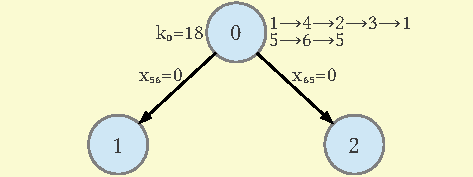
\includegraphics{kepek/alkorut.pdf}
\end{figure}

Most felírjuk az $1$ gráfponthoz tartozó táblát. Ehhez a kezdeti $T$ táblában beírunk a $t_{5,6}$ helyre egy $M$-et, jelezve hogy tiltott, majd sor-oszlop redukció után címkézünk:
\begin{center}
\begin{tikzpicture}[
    covered/.style={decorate, draw=black, decoration={complete sines,amplitude=5pt, segment length=15pt}},
    cell/.style={nodes={rectangle,draw=black}},
    space/.style={matrix of nodes,row sep=-\pgflinewidth,column sep=-\pgflinewidth},
    text height = 3mm, anchor = center, text width = 7mm, nodes in empty cells,row sep=-\pgflinewidth,column sep=-\pgflinewidth,
]
    \matrix (magic) [matrix of nodes,
          nodes = {draw},
          text centered
    ] at (0,0)
    {%
        \phantom{$0$} & $3$ & $7$ & $0$ & $8$ & $11$\\
        $9$ & \phantom{$0$} & $0$ & $10$ & $7$ & $3$\\
        $0$ & $5$ & \phantom{$0$} & $2$ & $9$ & $12$\\
        $3$ & $2$ & $8$ & \phantom{$0$}& $10$ & $0$\\
        $7$ & $10$ & $3$ & $0$ &\phantom{$0$} & $M$\\
        $5$ & $0$ & $8$ & $10$ & $0$ &\phantom{$0$}\\
    };
    \draw[thick] (magic-1-1.north west) -- (magic-6-6.south east);
    
    \matrix (magic_right) [matrix of nodes,
          nodes = {draw},
          text centered
    ] at (4,0)
    {%
        $+4$\\
        \phantom{$0$}\\
        \phantom{$0$}\\
        \phantom{$0$}\\
        $+s$\\
        \phantom{$0$}\\
    };
    
        \matrix (magic_bottom) [matrix of nodes,
          nodes = {draw},
          text centered
    ] at (0,-2.5)
    {%
        \phantom{$0$} & \phantom{$0$} & \phantom{$0$} & $+5$ & \phantom{$0$} & \phantom{$0$}\\
    };
    
    \node[text width = 1cm] at (4.1,-2.5) {$\varepsilon=3$};
    \draw[covered] (magic-2-1.west) -- (magic-2-6.east);
    \draw[covered] (magic-3-1.west) -- (magic-3-6.east);
    \draw[covered] (magic-4-1.west) -- (magic-4-6.east);
    \draw[covered] (magic-6-1.west) -- (magic-6-6.east);
    \draw[covered] (magic-1-4.north) -- (magic-6-4.south);
\end{tikzpicture}
\end{center}

Itt megint lefedtünk, az új tábla a következő:
\begin{center}
\begin{tikzpicture}[
    covered/.style={decorate, draw=black, decoration={complete sines,amplitude=5pt, segment length=15pt}},
    cell/.style={nodes={rectangle,draw=black}},
    space/.style={matrix of nodes,row sep=-\pgflinewidth,column sep=-\pgflinewidth},
    text height = 3mm, anchor = center, text width = 7mm, nodes in empty cells,row sep=-\pgflinewidth,column sep=-\pgflinewidth,
]
    \matrix (magic) [matrix of nodes,
          nodes = {draw},
          text centered
    ] at (0,0)
    {%
        \phantom{$0$} & $0$ & $4$ & $0$ & $5$ & $8$\\
        $9$ & \phantom{$0$} & $0$ & $13$ & $7$ & $3$\\
        $0$ & $5$ & \phantom{$0$} & $5$ & $9$ & $11$\\
        $3$ & $2$ & $8$ & \phantom{$0$}& $10$ & $0$\\
        $4$ & $7$ & $0$ & $0$ &\phantom{$0$} & $M$\\
        $5$ & $0$ & $8$ & $13$ & $0$ &\phantom{$0$}\\
    };
    \draw[thick] (magic-1-1.north west) -- (magic-6-6.south east);
    \draw[thick] (-1.47,1.5) circle(2.5mm);
    \draw[thick] (2.45,-0.3) circle(2.5mm);
    \draw[thick] (-0.49,0.9) circle(2.5mm);
    \draw[thick] (-2.45,0.3) circle(2.5mm);
    \draw[thick] (0.49,-0.9) circle(2.5mm);
    \draw[thick] (1.47,-1.5) circle(2.5mm);
\end{tikzpicture}
\end{center}

Az észak-nyugati sarok módszer most jó eredményt adott. A körutak most: $1\xrightarrow{5}2\xrightarrow{3}3\xrightarrow{1}1$ és $4\xrightarrow{2}6\xrightarrow{3}5\xrightarrow{4}4$. Az utak összsúlya $k_1=18$.

s.í.t.
\end{megoldas}

\subsection{Körút építő algoritmus}

\firstline A módszer a körutat lépésenként fogjuk felépíteni.

\feladatszam Adott egy 5 városú utazó ügynök probléma, az alábbi költségmátrixszal:
\begin{center}
\begin{tikzpicture}[
    covered/.style={decorate, draw=black, decoration={complete sines,amplitude=5pt, segment length=15pt}},
    cell/.style={nodes={rectangle,draw=black}},
    space/.style={matrix of nodes,row sep=-\pgflinewidth,column sep=-\pgflinewidth},
    text height = 3mm, anchor = center, text width = 7mm, nodes in empty cells,row sep=-\pgflinewidth,column sep=-\pgflinewidth,
]
    \matrix (magic) [matrix of nodes,
          nodes = {draw},
          text centered
    ]
    {%
        \phantom{$0$} & $8$ & $3$ & $7$ & $4$\\
        $13$ & \phantom{$0$} & $4$ & $5$ & $1$\\
        $2$ & $6$ & \phantom{$0$} & $5$ & $3$\\
        $8$ & $5$ & $1$ & \phantom{$0$}& $7$\\
        $7$ & $4$ & $8$ & $2$ &\phantom{$0$}\\
    };
    \draw[thick] (magic-1-1.north west) -- (magic-5-5.south east);
    \node[text width=1cm] at (-2.8,0) {$C_0=$};
\end{tikzpicture}
\end{center}

\begin{megoldas}
\begin{center}
\begin{tikzpicture}[
    covered/.style={decorate, draw=black, decoration={complete sines,amplitude=5pt, segment length=15pt}},
    cell/.style={nodes={rectangle,draw=black}},
    space/.style={matrix of nodes,row sep=-\pgflinewidth,column sep=-\pgflinewidth},
    text height = 3mm, anchor = center, text width = 7mm, nodes in empty cells,row sep=-\pgflinewidth,column sep=-\pgflinewidth,
]
    \matrix (magic) [matrix of nodes,
          nodes = {draw},
          text centered
    ]
    {%
        \phantom{$0$} & $3$ & $0$ & $4$ & $1$\\
        $12$ & \phantom{$0$} & $3$ & $4$ & $0$\\
        $0$ & $2$ & \phantom{$0$} & $3$ & $1$\\
        $7$ & $2$ & $0$ & \phantom{$0$}& $6$\\
        $5$ & $0$ & $6$ & $0$ &\phantom{$0$}\\
    };
    \draw[thick] (magic-1-1.north west) -- (magic-5-5.south east);
    \node[text width=1cm] at (-2.8,0) {$\widehat{C}_0=$};
\end{tikzpicture}
\end{center}

Az $u$ és $v$ vektorok elemeinek összege pedig $11$. Ez lesz a $k_0$ értékünk. A továbblépéshez megkeressük a legkisebb költségű $x_{i,j}$ elemet, ahol a $\widehat{c}_{i,j}=0$. Itt két ilyen van, így választanunk egyet. Most a $x_{2,5}$ szerint haladunk tovább:
\begin{figure}[H]
\centering
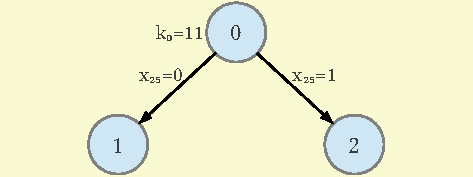
\includegraphics{kepek/korutepito.pdf}
\end{figure}

Ha a $2\rightarrow 5$ utazást megtiltjuk, akkor $c_{2,5} = M$. Ekkor a költségmátrix: 
\begin{center}
\begin{tikzpicture}[
    covered/.style={decorate, draw=black, decoration={complete sines,amplitude=5pt, segment length=15pt}},
    cell/.style={nodes={rectangle,draw=black}},
    space/.style={matrix of nodes,row sep=-\pgflinewidth,column sep=-\pgflinewidth},
    text height = 3mm, anchor = center, text width = 7mm, nodes in empty cells,row sep=-\pgflinewidth,column sep=-\pgflinewidth,
]
    \matrix (magic) [matrix of nodes,
          nodes = {draw},
          text centered
    ]
    {%
        \phantom{$0$} & $8$ & $3$ & $7$ & $4$\\
        $13$ & \phantom{$0$} & $4$ & $5$ & $M$\\
        $2$ & $6$ & \phantom{$0$} & $5$ & $3$\\
        $8$ & $5$ & $1$ & \phantom{$0$}& $7$\\
        $7$ & $4$ & $8$ & $2$ &\phantom{$0$}\\
    };
    \draw[thick] (magic-1-1.north west) -- (magic-5-5.south east);
    \node[text width=1cm] at (-2.8,0) {$C_1=$};
\end{tikzpicture}
\end{center}

Az $u$ és $v$ vektorok összege $\lVert u\rVert+\lVert v\rVert=15$. Tehát $k_1=15$, most pedig visszalépünk a 0 gráfpontba. Ha $2\rightarrow 5$ utazást elfogadjuk, akkor a fordított irányt tiltanunk kell és a 2. sort és az 5. oszlopot törölni. Így a $C_2$ költségmátrix a következő:
\begin{center}
\begin{tikzpicture}[
    covered/.style={decorate, draw=black, decoration={complete sines,amplitude=5pt, segment length=15pt}},
    cell/.style={nodes={rectangle,draw=black}},
    space/.style={matrix of nodes,row sep=-\pgflinewidth,column sep=-\pgflinewidth},
    text height = 3mm, anchor = center, text width = 7mm, nodes in empty cells,row sep=-\pgflinewidth,column sep=-\pgflinewidth,
]
    \matrix (magic) [matrix of nodes,
          nodes = {draw},
          text centered
    ]
    {%
        \phantom{$0$} & $8$ & $3$ & $7$ & \phantom{$0$}\\
        \phantom{$0$} & \phantom{$0$} & \phantom{$0$} & \phantom{$0$} & \phantom{$0$}\\
        $2$ & $6$ & \phantom{$0$} & $5$ & \phantom{$0$}\\
        $8$ & $5$ & $1$ & \phantom{$0$}& \phantom{$0$}\\
        $7$ & $M$ & $8$ & $2$ &\phantom{$0$}\\
    };
    \draw[thick] (magic-1-1.north west) -- (magic-5-5.south east);
    \draw[thick,covered] (magic-1-5.north) -- (magic-5-5.south);
    \draw[thick,covered] (magic-2-1.west) -- (magic-2-5.east);
    \node[text width=1cm] at (-2.8,0) {$C_2=$};
\end{tikzpicture}
\end{center}
\end{megoldas}

\begin{megoldas}
Az $\lVert u\rVert+\lVert v\rVert=12$, viszont itt ehhez hozzá kell adni $c_{2,5}$-t, így $k_2=13$. Mivel ez jobb mint a másik ág értéke, így inkább erre haladunk tovább. Mivel továbbágazzuk a gráfot, így szükség van a $\widehat{C}_2$ mátrixra:
\begin{center}
\begin{tikzpicture}[
    covered/.style={decorate, draw=black, decoration={complete sines,amplitude=5pt, segment length=15pt}},
    cell/.style={nodes={rectangle,draw=black}},
    space/.style={matrix of nodes,row sep=-\pgflinewidth,column sep=-\pgflinewidth},
    text height = 3mm, anchor = center, text width = 7mm, nodes in empty cells,row sep=-\pgflinewidth,column sep=-\pgflinewidth,
]
    \matrix (magic) [matrix of nodes,
          nodes = {draw},
          text centered
    ]
    {%
        \phantom{$0$} & $1$ & $0$ & $4$ & \phantom{$0$}\\
        \phantom{$0$} & \phantom{$0$} & \phantom{$0$} & \phantom{$0$} & \phantom{$0$}\\
        $0$ & $0$ & \phantom{$0$} & $3$ & \phantom{$0$}\\
        $7$ & $0$ & $0$ & \phantom{$0$}& \phantom{$0$}\\
        $5$ & $M$ & $6$ & $0$ &\phantom{$0$}\\
    };
    \draw[thick] (magic-1-1.north west) -- (magic-5-5.south east);
    \draw[thick,covered] (magic-1-5.north) -- (magic-5-5.south);
    \draw[thick,covered] (magic-2-1.west) -- (magic-2-5.east);
    \node[text width=1cm] at (-2.8,0) {$\widehat{C}_2=$};
\end{tikzpicture}
\end{center}

Ismét két legolcsóbb lehetőségünk van, most a $x_{3,1}$-et választjuk.
\begin{figure}[H]
\centering
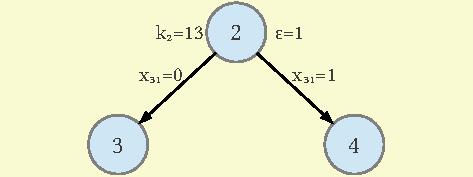
\includegraphics{kepek/korutepito2.pdf}
\end{figure}
\begin{multicols}{2}
\begin{center}
\begin{tikzpicture}[
    covered/.style={decorate, draw=black, decoration={complete sines,amplitude=5pt, segment length=15pt}},
    cell/.style={nodes={rectangle,draw=black}},
    space/.style={matrix of nodes,row sep=-\pgflinewidth,column sep=-\pgflinewidth},
    text height = 3mm, anchor = center, text width = 7mm, nodes in empty cells,row sep=-\pgflinewidth,column sep=-\pgflinewidth,
]
    \matrix (magic) [matrix of nodes,
          nodes = {draw},
          text centered
    ]
    {%
        \phantom{$0$} & $8$ & $3$ & $7$ & \phantom{$0$}\\
        \phantom{$0$} & \phantom{$0$} & \phantom{$0$} & \phantom{$0$} & \phantom{$0$}\\
        $M$ & $6$ & \phantom{$0$} & $5$ & \phantom{$0$}\\
        $8$ & $5$ & $1$ & \phantom{$0$}& \phantom{$0$}\\
        $7$ & $M$ & $8$ & $2$ &\phantom{$0$}\\
    };
    \draw[thick] (magic-1-1.north west) -- (magic-5-5.south east);
    \draw[thick,covered] (magic-1-5.north) -- (magic-5-5.south);
    \draw[thick,covered] (magic-2-1.west) -- (magic-2-5.east);
    \node[text width=1cm] at (-2.8,0) {$C_3=$};
\end{tikzpicture}

$\lVert u\rVert+\lVert v\rVert=17$\\$k_3=18$
\end{center}

\begin{center}
\begin{tikzpicture}[
    covered/.style={decorate, draw=black, decoration={complete sines,amplitude=5pt, segment length=15pt}},
    cell/.style={nodes={rectangle,draw=black}},
    space/.style={matrix of nodes,row sep=-\pgflinewidth,column sep=-\pgflinewidth},
    text height = 3mm, anchor = center, text width = 7mm, nodes in empty cells,row sep=-\pgflinewidth,column sep=-\pgflinewidth,
]
    \matrix (magic) [matrix of nodes,
          nodes = {draw},
          text centered
    ]
    {%
        \phantom{$0$} & $8$ & $M$ & $7$ & \phantom{$0$}\\
        \phantom{$0$} & \phantom{$0$} & \phantom{$0$} & \phantom{$0$} & \phantom{$0$}\\
        \phantom{$0$} & \phantom{$0$} & \phantom{$0$} & \phantom{$0$} & \phantom{$0$}\\
        \phantom{$0$} & $5$ & $1$ & \phantom{$0$}& \phantom{$0$}\\
        \phantom{$0$} & $M$ & $8$ & $2$ &\phantom{$0$}\\
    };
    \draw[thick] (magic-1-1.north west) -- (magic-5-5.south east);
    \draw[thick,covered] (magic-1-5.north) -- (magic-5-5.south);
    \draw[thick,covered] (magic-1-1.north) -- (magic-5-1.south);
    \draw[thick,covered] (magic-2-1.west) -- (magic-2-5.east);
    \draw[thick,covered] (magic-3-1.west) -- (magic-3-5.east);
    \node[text width=1cm] at (-2.8,0) {$C_4=$};
\end{tikzpicture}

$\lVert u\rVert+\lVert v\rVert=11$\\$k_4=14$
\end{center}
\end{multicols}

Mivel a 4-es gráfpontban kedvezőbb az $k_4$ érték, ezért arra megyünk tovább.
\begin{center}
\begin{tikzpicture}[
    covered/.style={decorate, draw=black, decoration={complete sines,amplitude=5pt, segment length=15pt}},
    cell/.style={nodes={rectangle,draw=black}},
    space/.style={matrix of nodes,row sep=-\pgflinewidth,column sep=-\pgflinewidth},
    text height = 3mm, anchor = center, text width = 7mm, nodes in empty cells,row sep=-\pgflinewidth,column sep=-\pgflinewidth,
]
    \matrix (magic) [matrix of nodes,
          nodes = {draw},
          text centered
    ]
    {%
        \phantom{$0$} & $0$ & $M$ & $0$ & \phantom{$0$}\\
        \phantom{$0$} & \phantom{$0$} & \phantom{$0$} & \phantom{$0$} & \phantom{$0$}\\
        \phantom{$0$} & \phantom{$0$} & \phantom{$0$} & \phantom{$0$} & \phantom{$0$}\\
        \phantom{$0$} & $3$ & $0$ & \phantom{$0$}& \phantom{$0$}\\
        \phantom{$0$} & $M$ & $6$ & $0$ &\phantom{$0$}\\
    };
    \draw[thick] (magic-1-1.north west) -- (magic-5-5.south east);
    \draw[thick,covered] (magic-1-5.north) -- (magic-5-5.south);
    \draw[thick,covered] (magic-1-1.north) -- (magic-5-1.south);
    \draw[thick,covered] (magic-2-1.west) -- (magic-2-5.east);
    \draw[thick,covered] (magic-3-1.west) -- (magic-3-5.east);
    \node[text width=1cm] at (-2.8,0) {$\widehat{C}_4=$};
\end{tikzpicture}
\end{center}

Most csak egyetlen opciónk van, az $x_{4,3}$:
\begin{figure}[H]
\centering
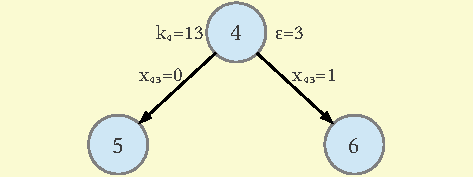
\includegraphics{kepek/korutepito3.pdf}
\end{figure}
\end{megoldas}

\begin{megoldas}
\begin{multicols}{2}
\begin{center}
\begin{tikzpicture}[
    covered/.style={decorate, draw=black, decoration={complete sines,amplitude=5pt, segment length=15pt}},
    cell/.style={nodes={rectangle,draw=black}},
    space/.style={matrix of nodes,row sep=-\pgflinewidth,column sep=-\pgflinewidth},
    text height = 3mm, anchor = center, text width = 7mm, nodes in empty cells,row sep=-\pgflinewidth,column sep=-\pgflinewidth,
]
    \matrix (magic) [matrix of nodes,
          nodes = {draw},
          text centered
    ]
    {%
        \phantom{$0$} & $8$ & $M$ & $7$ & \phantom{$0$}\\
        \phantom{$0$} & \phantom{$0$} & \phantom{$0$} & \phantom{$0$} & \phantom{$0$}\\
        \phantom{$0$} & \phantom{$0$} & \phantom{$0$} & \phantom{$0$} & \phantom{$0$}\\
        \phantom{$0$} & $5$ & $M$ & \phantom{$0$}& \phantom{$0$}\\
        \phantom{$0$} & $M$ & $8$ & $2$ &\phantom{$0$}\\
    };
    \draw[thick] (magic-1-1.north west) -- (magic-5-5.south east);
    \draw[thick,covered] (magic-1-5.north) -- (magic-5-5.south);
    \draw[thick,covered] (magic-1-1.north) -- (magic-5-1.south);
    \draw[thick,covered] (magic-2-1.west) -- (magic-2-5.east);
    \draw[thick,covered] (magic-3-1.west) -- (magic-3-5.east);
    \node[text width=1cm] at (-2.8,0) {$C_5=$};
\end{tikzpicture}

$\lVert u\rVert+\lVert v\rVert=10$\\$k_5=13$
\end{center}

\begin{center}
\begin{tikzpicture}[
    covered/.style={decorate, draw=black, decoration={complete sines,amplitude=5pt, segment length=15pt}},
    cell/.style={nodes={rectangle,draw=black}},
    space/.style={matrix of nodes,row sep=-\pgflinewidth,column sep=-\pgflinewidth},
    text height = 3mm, anchor = center, text width = 7mm, nodes in empty cells,row sep=-\pgflinewidth,column sep=-\pgflinewidth,
]
    \matrix (magic) [matrix of nodes,
          nodes = {draw},
          text centered
    ]
    {%
        \phantom{$0$} & $8$ & \phantom{$0$} & $7$ & \phantom{$0$}\\
        \phantom{$0$} & \phantom{$0$} & \phantom{$0$} & \phantom{$0$} & \phantom{$0$}\\
        \phantom{$0$} & \phantom{$0$} & \phantom{$0$} & \phantom{$0$} & \phantom{$0$}\\
        \phantom{$0$} & \phantom{$0$} & \phantom{$0$} & \phantom{$0$}& \phantom{$0$}\\
        \phantom{$0$} & $M$ & \phantom{$0$} & $2$ &\phantom{$0$}\\
    };
    \draw[thick] (magic-1-1.north west) -- (magic-5-5.south east);
    \draw[thick,covered] (magic-1-5.north) -- (magic-5-5.south);
    \draw[thick,covered] (magic-1-1.north) -- (magic-5-1.south);
    \draw[thick,covered] (magic-1-3.north) -- (magic-5-3.south);
    \draw[thick,covered] (magic-2-1.west) -- (magic-2-5.east);
    \draw[thick,covered] (magic-3-1.west) -- (magic-3-5.east);
    \draw[thick,covered] (magic-4-1.west) -- (magic-4-5.east);
    \node[text width=1cm] at (-2.8,0) {$C_6=$};
\end{tikzpicture}

$\lVert u\rVert+\lVert v\rVert=10$\\$z_6=14$
\end{center}
\end{multicols}

Most így kaptunk egy lehetséges megoldást, de az alsó határokat is megnézve nem biztos hogy ez az optimális. A 3-mas gráfpontból továbbmenve jobb megoldást biztosan nem kaphatunk, az 5-ösből viszont még lehetséges. Ezért lássuk a {$\widehat{C}_5$} mátrixot:
\begin{center}
\begin{tikzpicture}[
    covered/.style={decorate, draw=black, decoration={complete sines,amplitude=5pt, segment length=15pt}},
    cell/.style={nodes={rectangle,draw=black}},
    space/.style={matrix of nodes,row sep=-\pgflinewidth,column sep=-\pgflinewidth},
    text height = 3mm, anchor = center, text width = 7mm, nodes in empty cells,row sep=-\pgflinewidth,column sep=-\pgflinewidth,
]
    \matrix (magic) [matrix of nodes,
          nodes = {draw},
          text centered
    ]
    {%
        \phantom{$0$} & $1$ & $M$ & $0$ & \phantom{$0$}\\
        \phantom{$0$} & \phantom{$0$} & \phantom{$0$} & \phantom{$0$} & \phantom{$0$}\\
        \phantom{$0$} & \phantom{$0$} & \phantom{$0$} & \phantom{$0$} & \phantom{$0$}\\
        \phantom{$0$} & $0$ & $M$ & \phantom{$0$}& \phantom{$0$}\\
        \phantom{$0$} & $M$ & $6$ & $0$ &\phantom{$0$}\\
    };
    \draw[thick] (magic-1-1.north west) -- (magic-5-5.south east);
    \draw[thick,covered] (magic-1-5.north) -- (magic-5-5.south);
    \draw[thick,covered] (magic-1-1.north) -- (magic-5-1.south);
    \draw[thick,covered] (magic-2-1.west) -- (magic-2-5.east);
    \draw[thick,covered] (magic-3-1.west) -- (magic-3-5.east);
    \node[text width=1cm] at (-2.8,0) {$\widehat{C}_5=$};
\end{tikzpicture}
\end{center}

Az $x_{5,4}$-et választjuk:
\begin{figure}[H]
\centering
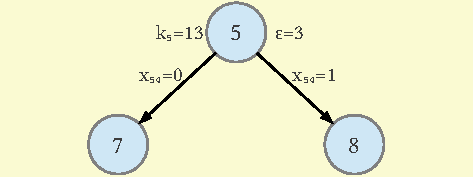
\includegraphics{kepek/korutepito4.pdf}
\end{figure}

\begin{multicols}{2}
\begin{center}
\begin{tikzpicture}[
    covered/.style={decorate, draw=black, decoration={complete sines,amplitude=5pt, segment length=15pt}},
    cell/.style={nodes={rectangle,draw=black}},
    space/.style={matrix of nodes,row sep=-\pgflinewidth,column sep=-\pgflinewidth},
    text height = 3mm, anchor = center, text width = 7mm, nodes in empty cells,row sep=-\pgflinewidth,column sep=-\pgflinewidth,
]
    \matrix (magic) [matrix of nodes,
          nodes = {draw},
          text centered
    ]
    {%
        \phantom{$0$} & $8$ & $M$ & $7$ & \phantom{$0$}\\
        \phantom{$0$} & \phantom{$0$} & \phantom{$0$} & \phantom{$0$} & \phantom{$0$}\\
        \phantom{$0$} & \phantom{$0$} & \phantom{$0$} & \phantom{$0$} & \phantom{$0$}\\
        \phantom{$0$} & $5$ & $M$ & \phantom{$0$}& \phantom{$0$}\\
        \phantom{$0$} & $M$ & $8$ & $M$ &\phantom{$0$}\\
    };
    \draw[thick] (magic-1-1.north west) -- (magic-5-5.south east);
    \draw[thick,covered] (magic-1-5.north) -- (magic-5-5.south);
    \draw[thick,covered] (magic-1-1.north) -- (magic-5-1.south);
    \draw[thick,covered] (magic-2-1.west) -- (magic-2-5.east);
    \draw[thick,covered] (magic-3-1.west) -- (magic-3-5.east);
    \node[text width=1cm] at (-2.8,0) {$C_7=$};
\end{tikzpicture}

$\lVert u\rVert+\lVert v\rVert=20$\\$k_7=23$
\end{center}

\begin{center}
\begin{tikzpicture}[
    covered/.style={decorate, draw=black, decoration={complete sines,amplitude=5pt, segment length=15pt}},
    cell/.style={nodes={rectangle,draw=black}},
    space/.style={matrix of nodes,row sep=-\pgflinewidth,column sep=-\pgflinewidth},
    text height = 3mm, anchor = center, text width = 7mm, nodes in empty cells,row sep=-\pgflinewidth,column sep=-\pgflinewidth,
]
    \matrix (magic) [matrix of nodes,
          nodes = {draw},
          text centered
    ]
    {%
        \phantom{$0$} & $8$ & $M$ & \phantom{$0$} & \phantom{$0$}\\
        \phantom{$0$} & \phantom{$0$} & \phantom{$0$} & \phantom{$0$} & \phantom{$0$}\\
        \phantom{$0$} & \phantom{$0$} & \phantom{$0$} & \phantom{$0$} & \phantom{$0$}\\
        \phantom{$0$} & $5$ & $M$ & \phantom{$0$}& \phantom{$0$}\\
        \phantom{$0$} & \phantom{$0$} & \phantom{$0$} & \phantom{$0$} & \phantom{$0$}\\
    };
    \draw[thick] (magic-1-1.north west) -- (magic-5-5.south east);
    \draw[thick,covered] (magic-1-5.north) -- (magic-5-5.south);
    \draw[thick,covered] (magic-1-1.north) -- (magic-5-1.south);
    \draw[thick,covered] (magic-1-4.north) -- (magic-5-4.south);
    \draw[thick,covered] (magic-2-1.west) -- (magic-2-5.east);
    \draw[thick,covered] (magic-3-1.west) -- (magic-3-5.east);
    \draw[thick,covered] (magic-5-1.west) -- (magic-5-5.east);
    \node[text width=1cm] at (-2.8,0) {$C_8=$};
\end{tikzpicture}

$\lVert u\rVert+\lVert v\rVert=13$\\$z_8=18$
\end{center}
\end{multicols}

Jól látható, hogy ez rosszabb, mint a $z_6$ érték, tehát ez nem lehet optimális megoldás. Tehát az egyetlen optimum a 6-os gráfpontnál található, ez pedig:
\begin{figure}[H]
\centering
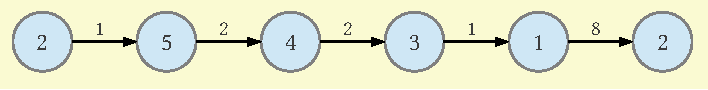
\includegraphics{kepek/korutepito5.pdf}
\end{figure}
\end{megoldas}

\begin{megoldas}
Ezzel megoldottuk a feladatot, a teljesség kedvéért még lerajzoljuk a teljes gráfot:
\begin{figure}[H]
\centering
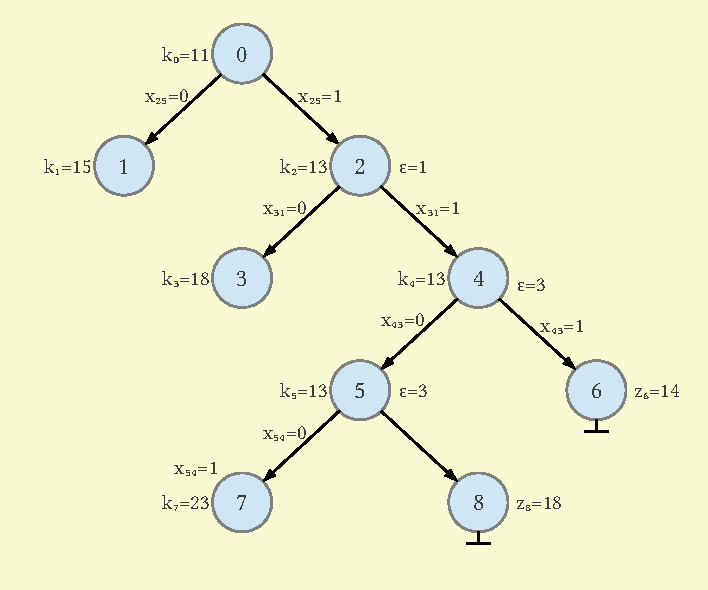
\includegraphics{kepek/korutepito6.pdf}
\end{figure}

Innen nagyon jól láthatjuk, hogy az 1-es, 3-mas és 7-es gráfpontokból továbbhaladva sem kaphatunk a $z_6$ értéknél kisebbet.
\end{megoldas}
\end{document}